\documentclass[11pt]{article}
\usepackage{amsmath,amssymb}
\usepackage{graphicx}
\usepackage[margin=1in]{geometry}
\usepackage{xcolor}
\usepackage{hyperref}
\usepackage{amsmath}
\usepackage{empheq}

\newcommand{\mga}[1]{{\color[rgb]{0.8,0,0}#1}}
\newcommand{\mgacom}[1]{\textsf{\color[rgb]{0.75,0,0}[\textsuperscript{MGA} #1]}}

\newcommand{\AH}[1]{{\color{cyan}#1}}
\newcommand{\AHcom}[1]{\textsf{\color{cyan}{\textsuperscript{AH}#1}}}

\newcommand{\LB}[1]{{\color{brown}#1}}
\newcommand{\LBcom}[1]{\textsf{\color{brown}[\textsuperscript{LB}#1]}}

\newcommand{\JS}[1]{{\color{violet}#1}}
\newcommand{\JScom}[1]{\textsf{\color{violet} [\textsuperscript{JS}#1]}}

% Greek alphabet: 2 letter abbreviations
\newcommand{\al}{\alpha}
\newcommand{\be}{\beta}
\newcommand{\ga}{\gamma}
\newcommand{\Ga}{\Gamma}
\newcommand{\de}{\delta}
\newcommand{\De}{\Delta}
\newcommand{\ep}{\varepsilon}

\newcommand{\eps}{\epsilon}
\newcommand{\ze}{\zeta}
\newcommand{\ka}{\kappa}
\newcommand{\la}{\lambda}
\newcommand{\La}{\Lambda}
\newcommand{\ph}{\varphi}
\newcommand{\del}{\nabla}
\newcommand{\si}{\sigma}
\newcommand{\Si}{\Sigma}
\renewcommand{\th}{\theta}   % LaTeX: \th already defined
\newcommand{\Up}{\Upsilon}
\newcommand{\om}{\omega}
\newcommand{\Om}{\Omega}
% end Greek alphabet

% Other abbreviations
\newcommand{\p}{\partial}
\newcommand{\Qstar}{{\ensuremath{Q^*}}}
\newcommand{\aQstar}{{\ensuremath{a_{Q^*}}}}
\newcommand{\aQstarmax}{{\ensuremath{a_{Q^*}^\text{max}}}}

\begin{document}

\section{State of the art}

Equations to be solved: 

\begin{subequations}\label{eq:front_system}
\begin{empheq}[left=\empheqlbrace]{align}
&\partial_x\Big(u(x)n_B(x)\Big) = 0 ,
\label{eq:baryon_conservation}\\
&\partial_x\Big(h(x)u^2(x)+P(x)\Big) = 0 ,
\label{eq:momentum_conservation}\\
&\partial_x\Big(D_K\partial_x n_K(x)-u(x)n_K(x)\Big) = \Gamma_K(n_K) ,
\label{eq:kaonness_diffusion}\\
&\partial_x\Big(h(x)u(x)\gamma(x)\Big) = 0 .
\label{eq:energy_conservation}
\end{empheq}
\end{subequations}
%\mgacom{Are we going to replace $a$ with $n_K$ to avoid having to look ahead to $x=\infty$?} \JScom{Using $n_K$ would be cleaner and Alex is using that I think. My code is using $a$, and it's a working code and it would be painful for me to change to $n_K$. I'm inclined not to change my code unless Alex's result disagree with mine.} 
%\mgacom{It's just a rescaling. Could we redefine $a\equiv n_K/n_B(0^+)$? Is that any different from the current definition, given the vagueness about what ``$\mu_Q$'' means in the formulas for $\mathcal{R}$?}
%\JScom{Numerically I don't think there would be a difference at all, since $n_B(x>0)$ is roughly constant ($n_B$ varies only by $10^{-10}$.)}
Integrate across $0$ and the jump conditions are:
\begin{subequations}\label{eq:jump_conditions}
\begin{empheq}[left=\empheqlbrace]{align}
& j_B = n_B^- u_- = n_B^{+} u_{+}
\label{eq:jump_baryon}\\
& \Pi = h_- u_-^2 + P_- = h_{+}u_{+}^2 + P_{+}
\label{eq:jump_momentum}\\
& D_K(T_{+})\frac{dn_K}{dx}(0^+) - u_{+}n_K^{+} = -u_- n_K^-
\label{eq:jump_kaonness}\\
& E = h_- u_- \gamma = h_{+}u_{+}\gamma
\label{eq:jump_energy}
\end{empheq}
\end{subequations}
and at quark matter side $0<x<\infty$, we expect boundary conditions for $a$ as:
\begin{equation}
\left\{
\begin{aligned}
& a(0^+) = a_{Q^*} \\
& a(\infty) = 0 \\
\end{aligned}
\right.
\end{equation}

\subsection{Numerical strategy}

We integrate the three conservation equations Eqs.~\eqref{eq:baryon_conservation}\eqref{eq:momentum_conservation}\eqref{eq:energy_conservation}, to get first integrals, making ODE's into algebraic equations:
\begin{equation}
j_B=n_B u = \text{const},\qquad \Pi = hu^2 + P=\text{const},\qquad E = hu\gamma_u=\text{const}.
\end{equation}
So we end up with only one Kaon-ness 2nd order  Eq.~\eqref{eq:kaonness_diffusion} and three constraining algebraic equations. 
With nuclear matter side information, $T_N, n_B^N$, and input $a_{Q^*}$, then for a trial velocity, the jump conditions can determine the thermodynamic variables $\mu_B, \mu_K, T$ on $0^+$ side. 
%\mgacom{OK so there are 4 jump conditions and 5 things that need to be determined on the quark matter side: ($n_B(0^+)$, $n_K(0^+)$, $n'_K(0^+)$, $T_N(0^+)$, and $u_N(0^+)$) so one of them remains as a free parameter, and we take that to be $n_K(0^+)$.}\JScom{If we are taking the endothermic limit where $T_{Q^*} = 0$, which blows up $D_K$ because $D_K\sim T^{-5/3}$, then since $u_{Q^*}a_{Q^*}$ and $u_Na_N$ are both finite in Eq.~\eqref{eq:jump_kaonness}, we have to make $a'(0^+) = 0$, which would give us an $a_{Q^*}^{\rm max}$. This is another assumption used in deriving Eq.~\eqref{eq:uN_analytical}.} \mgacom{If $D_K$ is diverging at $x=0$ then I don't think (2c) is valid any more. Either we need to rethink the treatment of diffusion near such a singularity or we need to show that $1/D_K$ has other contributions that prevent it from going to zero.}
%\JScom{For diverging $D_K$, I think we can still solve the system of ODE by letting $a'(0^+) = 0$ so in this case Eq.~\eqref{eq:jump_kaonness} still holds. In general about diffusion of fermions, I'm probably wrong but I think at $T=0$, Pauli blocking would forbid fermions to scatter to lower momentum state. Incoming fermions all have momentum below fermi surface, but energy/momentum must conserve, so Pauli blocking forbids fermions to scatter and hence mean free path and collision time diverge, so does diffusion coefficient. Isn't this divergence inherent to $T=0$ fermi statistics?}

The remaining nontrivial spatial problem is the kaon-fraction profile
\(a(x)\). We solve it as a boundary-value/shooting problem on \(x>0\).
Defining
\begin{equation}
j_K(x) \equiv D_K(T)\frac{da}{dx}-u(x)a(x),
\end{equation}
the 2nd order ODE Eq.~\eqref{eq:kaonness_diffusion} becomes two first order ODE's
\begin{equation}
\left\{
\begin{aligned}
& \frac{dj_K}{dx}=\mathcal R(a),\\
& \frac{da}{dx} = \frac{j_K + ua}{D_K}
\end{aligned}
\right.
\end{equation}
velocity $u_N$, (under the hood it's $j_B$), is the shooting parameter, we hope to tune $u_N$ so that the following three conditions are met:
\begin{equation}
\left\{
\begin{aligned}
& a(0^+) = a_{Q^*}, \\
& j_K(0^+)=-u_N a_N, \\
& a(\infty) = 0.
\end{aligned}
\right.
\end{equation}
conservation of \(j_B,\Pi,E\) are enforced as well. This is the basic idea of numerical solver; there are some techniques used to improve the behavior. For details, see Sec.~\ref{sec:numerical_solver_implementation_details}.

\begin{figure}
    \centering
    \includegraphics[width=0.8\linewidth]{Hydrodynamical combustion/old/LTE_integrated.pdf}
    \caption{Velocity $u_N$ under extreme endothermic Eq.~\eqref{eq:uN_analytical}, local thermal equilibrium Eq.~\eqref{eq:uN_analytical_modified}, and numerical ODE's solution. Note that $a_{Q^*}^{\rm LTE}$ and $A$ hit 1 at the same time. }
    \label{fig:uN_contour}
\end{figure}

\subsection{Analytical Velocity Formula}
Under piecewise constant approximation, only three profiles $T(x), \mu_K(x), a(x)$ have non-trivial dependence on $x$, we get:
\begin{equation}
u_N^2
=
\frac{
54\pi^{7/3}
}{
7\sqrt{2}\,h_D\,\alpha_s^{5/3}
}
\frac{\gamma\cdot 
a_{Q^*}^{7/3}
}{
\mu_B^Q\cdot  a_N^2(1-a_{Q^*})(1+\xi a_{Q^*})
}.
\label{eq:uN_analytical}
\end{equation}
If $a_{Q^*}^{\rm max}$ starts with some non-zero $T(0^+)$, then denote $A$ the $a(0^+)$ that drives $T(0^+) = 0$, then we have a modified $u_N$:
\begin{equation}
u_N^2
=
\frac{
9\pi^{7/3}
}{
4\sqrt{2}\,h_D\,\alpha_s^{5/3}
}
\frac{
\gamma\cdot A^{7/3}
}{
\mu^Q_B\cdot a_N^2(1-a_{Q^*})(1+\xi a_{Q^*})
}
\left[
\frac{24}{7}
-3\left(1-\frac{a_{Q^*}^2}{A^2}\right)^{1/6}
-\frac{3}{7}
\left(1-\frac{a_{Q^*}^2}{A^2}\right)^{7/6}
\right].
\label{eq:uN_analytical_modified}
\end{equation}
If we set $a_{Q^*}^{\rm max} = A$, we get from Eq.~\eqref{eq:uN_analytical_modified} to Eq.~\eqref{eq:uN_analytical}. For derivations of these equations, see Sec.~\ref{sec:analytical_uN_derivation}.

\newpage\noindent
\mgacom{Added June 3, for discussion:}\\
{\bf The $D_K$ divergence problem:}\\
We found a divergence in $D_K$ as $x\to 0^+$ if we allow $\aQstar \to \aQstarmax$, because $\aQstarmax$ is the value at which $T(0^+)\to 0$. How do we deal with it?

\medskip\noindent {\bf What has gone wrong:} our equations stop being valid before $\aQstar$ reaches $\aQstarmax$.
Our equations assume that at each $x$, the quarks are in local thermal equilibrium, having a well defined temperature $T$ and a diffusion coeff $D_K(T)$ which is closely related to the mean free path $\la(T)$. When $T\to 0$, we find $D_K\to\infty$ which happens because $\la\to\infty$. 
But note that the mfp $\la$ is also the smallest distance scale on which we can treat the system as locally thermalized. Over distances smaller than $\la$ diffusion is not the main transport mechanism, particles can just move ballistically.

So in order for the diffusive equation to be a valid description of the movement of flavor, we need the distance scale on which $D_K$ varies to be much bigger than $\la$. Since $D_K$ mainly depends on $T$, this is the same as saying 
\begin{equation} \begin{array}{r@{\qquad}l}
r_T \gg \la & \text{local thermal equilibrium condition} \\[1ex] 
\text{where}\quad
r_T \sim \dfrac{T}{dT/dx}\quad\text{or}\quad 
\dfrac{D_K}{dD_K/dx} & \text{distance scale on which temperature or $D_K$ varies}
\end{array}
\end{equation}

\begin{figure}{h}
    \centering
    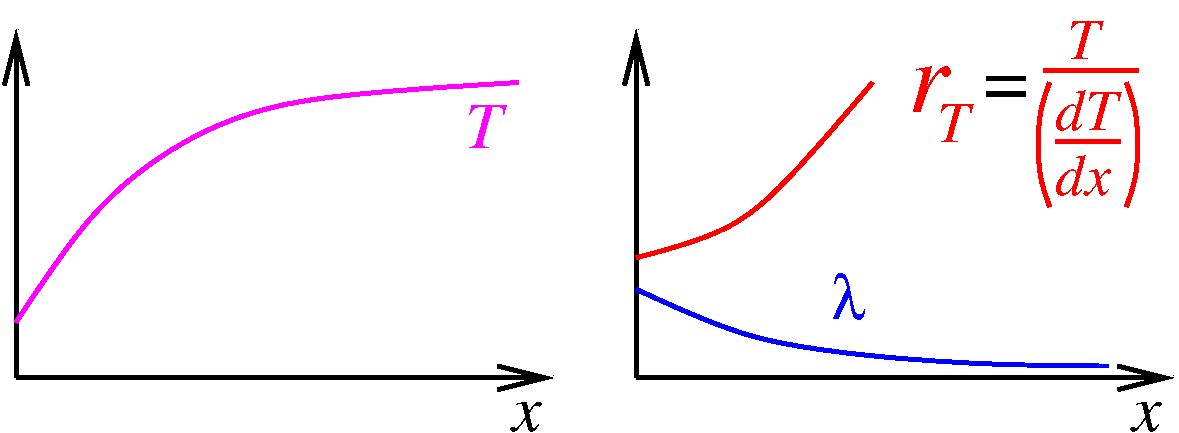
\includegraphics[width=0.5\hsize]{validity.pdf} 
    \caption{Caption}
    \label{fig:LTE_criterion}
\end{figure}

Usually the situation will be as illustrated in Fig.~\ref{fig:LTE_criterion}
where at all $x$ including $x=0$ the local thermal equilibrium condition is obeyed: temperature and $D_K$ varies slowly compared to the mfp, so $\la/r_T \ll 1$.

However, as $\aQstar\to \aQstarmax$, $r_T$ at $x=0$ gets smaller because $T$ drops towards zero (and $dT/dx$ presumably doesn't), also $\la$ rises (that's why $D_K$ gets large) so at some point as we keep raising $\aQstar$ we will find that the local thermal equilibrium condition is not valid at small $x$. At that point we have to stop raising $\aQstar$. In essence I am proposing an alternative, more restrictive, definition of $\aQstarmax$. 

\medskip\noindent{\bf Next steps:}\\
(1) We should estimate the new upper limit on $\aQstar$ \mga{and resultant boundary speed}.
For $\la$ there are different choices. One is just
$\la=3D_K$ (see \href{https://doi.org/10.1103/PhysRevD.48.2916}{Heiselberg and Pethick} eq~(36))).
\mga{If we define $r_T$ in terms of the spatial variation of $D_K$ then 
\begin{equation}
    \dfrac{\la}{r_T} = 3 D_K\dfrac{1}{D_K}\dfrac{dD_K}{dx} = 3\dfrac{dD_K}{dx}
    \label{mfp_criterion}
\end{equation}
and our equations are valid when this is much less than 1}
\mgacom{Jan, does this give a similar expression for $a_\Qstar^{\text{LTE}}$}?
\JScom{Yes, there's just a Jacobian in place. If we ignore sub-leading $T^2$ term in $D_K$, then %but the Jacobian can have negative sign, so we should take absolute value of $dD_K/dx$ or $dT/dx$ in the definition of $r_T$. The new definition of $r_T$ using $D_K$ is smaller than the definition of $r_T$ using $T$. Coming down to actual numbers, $\frac{1}{2}r_T < r_T^{\rm new} < \frac{3}{5}r_T$.}
\begin{equation}
\frac{D_K}{|D'_K|} = \frac{3}{5}\frac{T}{|T'|}
\end{equation}
this would lead to a smaller $a_{Q^*}^{\rm LTE}$.}
We want to know how fast the boundary can get if we let $\aQstar$ approach this new maximum value.
\\
(2) We should think about whether, if one could correctly treat the non-thermalized non-diffusive region at small $x$, the speed of the boundary could carry on getting larger? I don't think so, because the non-diffusive region still needs to be supplied with K-ness from the diffusive region, where $T$ is presumably not zero and $D_K$ is not particularly large.
But it's hard to prove that because to calculate $T$ we need to use our equations! 


\JS{
\medskip\noindent{\bf Addressing (1), local-thermal-equilibrium (LTE) bound on \(a_{Q^*}\).}

Let
\begin{equation}
A \equiv a(T_{Q*}=0)
\end{equation}
denote the old endpoint value at which the interface temperature would vanish.
Along the leading constant-pressure curve,
\begin{equation}
T^2(a)=C\left(A^2-a^2\right).
\end{equation}
Therefore, at the interface,
\begin{equation}
r_T(0^+)
\equiv
\frac{T}{|dT/dx|}
=
\frac{A^2-a_{Q^*}^2}{a_{Q^*}|da/dx|_{0^+}} .
\end{equation}
The kaon-current matching condition gives
\begin{equation}
D_K\frac{da}{dx}(0^+)
=
u_Qa_{Q^*}-u_Na_N .
\end{equation}
Using \(u_Q=a_Nu_N\), this becomes
\begin{equation}
\left|\frac{da}{dx}(0^+)\right|
=
\frac{u_Na_N(1-a_{Q^*})}{D_K}.
\end{equation}
Hence
\begin{equation}
r_T(0^+)
=
\frac{
D_K\left(A^2-a_{Q^*}^2\right)
}{
a_{Q^*}u_Na_N(1-a_{Q^*})
}.
\end{equation}
Now impose the local thermal equilibrium condition
\begin{equation}
\lambda_{\rm mfp}<r_T,
\qquad
\lambda_{\rm mfp}=3D_K .
\end{equation}
The diffusion coefficient cancels, giving
\begin{equation}
3u_Na_Na_{Q^*}(1-a_{Q^*})
<
A^2-a_{Q^*}^2 .
\end{equation}
Defining
\begin{equation}
\beta\equiv 3u_Na_N,
\end{equation}
we obtain
\begin{equation}
(1-\beta)a_{Q^*}^2+\beta a_{Q^*}-A^2<0 .
\end{equation}
Thus the local-thermal-equilibrium condition requires
\begin{equation}
a_{Q^*}
<
a_{Q^*}^{\rm LTE}
\equiv
\frac{
-\beta+
\sqrt{\beta^2+4(1-\beta)A^2}
}{
2(1-\beta)
},
\qquad
\beta=3u_Na_N .
\end{equation}
%In the special case \(\beta=1\), this expression should be replaced by its
%continuous limit,
%\begin{equation}
%a_{Q^*}^{\rm LTE}=A^2 .
% \end{equation}
For a slow front, \(\beta\ll1\), the bound is approximately
\begin{equation}
a_{Q^*}^{\rm LTE}
\simeq
A-\frac{\beta}{2}A(1-A)
=
A-\frac{3}{2}u_Na_NA(1-A).
\end{equation}
}
\mgacom{Nice expression! How fast can the boundary go if we impose this limit on $\aQstar$?}
\JScom{If we use $r_T = \frac{D_K}{|dD_K/dx|}$, and drop the sub-leading $T^2$ term in $D_K$, then we have
\begin{equation}
a_{Q^*}^{\rm LTE}
\simeq
A-\frac{5}{2}u_Na_NA(1-A).
\end{equation}
I'll try to implement this upper bound on $a_{Q^*}$ and produce a plot by Tuesday. Done, see Fig.~\ref{fig:uN_contour}}

\iffalse
\JScom{I looked more carefully at the derivation. Even we enforce 
\begin{equation}
\lambda_{\rm mfp} < \frac{r_T}{M}
\end{equation}
where $M$ is a very large number, we would still end up with
\begin{equation}
a_{Q^*}
<
a_{Q^*}^{\rm LTE}
\equiv
\frac{
-\beta+
\sqrt{\beta^2+4(1-\beta)A^2}
}{
2(1-\beta)
}
\end{equation}
Only difference is $\beta=5u_Na_N\cdot M$. So as long as $\beta < 1$, when $A = 0$, the new upper bound $a_{Q^*}^{\rm LTE}$ would hit 1 no matter what. 
}
\fi




\newpage

\section{Notes (Jun 1, 2026)}

\subsection{Finite-width local-thermal-equilibrium cutoff}

Let
\[
T_*\equiv T(0^+),\qquad T_Q\equiv T(\infty),\qquad
y\equiv\frac{T_*}{T_Q}.
\]
Define
\[
r_D=\frac{D_K}{|dD_K/dx|},\qquad
\ell_{\rm mfp}=3D_K,
\]
and impose
\[
\frac{\ell_{\rm mfp}}{r_D}<\varepsilon,
\]
where \(\varepsilon\ll1\) is the maximum tolerated local Knudsen number.

Near the cold interface, use
\[
D_K(T)=C_DT^{-5/3},\qquad
C_D=\frac{\pi q_D^{2/3}}{8N_f\alpha_s^2h_D}.
\]
Assume the temperature changes over a characteristic width \(\Delta x\):
\[
\max_x|T'(x)|\sim\frac{T_Q-T_*}{\Delta x}.
\]
The LTE condition becomes
\[
3\left|\frac{dD_K}{dx}\right|<\varepsilon
\]
and hence
\[
5C_D\frac{|T'|}{T^{8/3}}<\varepsilon.
\]
Evaluating the temperature factor at the cold side gives
\[
5C_D\frac{T_Q-T_*}{\Delta x\,T_*^{8/3}}<\varepsilon.
\]
Therefore,
\[
\frac{1-y}{y^{8/3}}<K,
\]
where
\[
\boxed{
K\equiv
\frac{\varepsilon\Delta x\,T_Q^{5/3}}{5C_D}
=
\frac{8N_f\alpha_s^2h_D}{5\pi q_D^{2/3}}
\varepsilon\Delta x\,T_Q^{5/3}.
}
\]
The limiting temperature ratio is the unique root \(0<y_{\rm LTE}<1\) of
\[
\boxed{Ky_{\rm LTE}^{8/3}+y_{\rm LTE}-1=0,}
\]
and LTE requires
\[
\boxed{T_*>T_Qy_{\rm LTE}.}
\]

Using
\[
T_Q=\frac{\sqrt{2}\,\bar\mu_B}{9\pi}A,
\]
we may write
\[
\boxed{
K=
\frac{8N_f\alpha_s^2h_D}{5\pi q_D^{2/3}}
\varepsilon\Delta x
\left(\frac{\sqrt{2}\,\bar\mu_BA}{9\pi}\right)^{5/3}.
}
\]
For \(K\gg1\),
\[
y_{\rm LTE}\simeq K^{-3/8},
\qquad
T_*^{\rm min}\simeq T_QK^{-3/8}.
\]
Since
\[
\frac{T_*^2}{T_Q^2}=1-\frac{a_{Q*}^2}{A^2},
\]
the LTE-limited composition is
\[
\boxed{
a_{Q*}^{\rm LTE}=A\sqrt{1-y_{\rm LTE}^2}.
}
\]

For \(\alpha_s=0.3\), \(h_D=1.81317\), \(N_f=3\),
\(\bar\mu_B=1200\,{\rm MeV}\), and \(\Delta x=500\,{\rm nm}\):
\[
\begin{array}{c|c|c|c}
A & \varepsilon & T_*^{\rm min}\,[{\rm MeV}] & a_{Q*}^{\rm LTE}\\ \hline
0.3 & 0.01 & 0.459 & 0.29990\\
0.5 & 0.01 & 0.557 & 0.49991\\
1.0 & 0.01 & 0.724 & 0.99993\\
1.0 & 0.10 & 0.306 & 0.99999
\end{array}
\]

\begin{figure}
    \centering
    \includegraphics[width=1.0\linewidth]{Hydrodynamical combustion/old/aQstar_scan.pdf}
    \caption{Caption}
    \label{fig:placeholder}
\end{figure}

\subsection{Ouyed Entropy Differential Equation from Energy Conservation}
\LB{
The point of the following is to show how the entropy equation in Ouyed comes from imposing energy conservation. Consider Eq.~\eqref{eq:energy_cons} at non-relativistic speeds ($\gamma=1$)
\begin{equation}
    \frac{\partial}{\partial x} (hu) = 0,
\end{equation}
where $h=\epsilon+P$ is the enthalpy. Use the thermodynamic relation $h= \sum_i\mu_i n_i + Ts$ to substitute for $h$
\begin{equation}
    \frac{\partial}{\partial x} \Big(\Big(\sum_i\mu_i n_i + Ts\Big)u\Big) = 0.
\end{equation}
Moving one term to the other side
\begin{equation}
     \frac{\partial}{\partial x}\Big(Tsu\Big) = -\frac{\partial}{\partial x} \Big(u\sum_i\mu_i n_i\Big).
\end{equation}
Assuming $\partial_x T=0$ \JScom{which isn't correct though}
\begin{equation}
     \frac{\partial}{\partial x}\Big(su\Big) = -\frac{1}{T}\frac{\partial}{\partial x} \Big(u\sum_i\mu_i n_i\Big).
\end{equation}
Assuming $\partial_x \mu_i =0$ and $\partial_x u = 0$ \JScom{$\mu_B$ is roughly constant, but $\mu_K$ certainly isn't}
\begin{equation}
     \frac{\partial}{\partial x}\Big(su\Big) = -\frac{1}{T}\sum_i\mu_i u\frac{\partial n_i}{\partial x}.
\end{equation}
Note that 
\begin{equation}
    \frac{dn}{dt} = \frac{\partial n}{\partial t} + u \frac{\partial n}{\partial x}.
\end{equation}
In the steady state approximation, $\frac{\partial n}{\partial t} =0$ so we are finally left with 
\begin{equation}
     \frac{\partial}{\partial x}\Big(su\Big) = -\frac{1}{T}\sum_i\mu_i \frac{dn_i}{dt},
\end{equation}
which matches what is in the 2010 paper with Ouyed~\cite{Niebergal:2010ds}.
}

\JS{
I also derived the entropy equation from energy conservation under piecewise constant approximation, also using the bag model EoS. It appears that entropy equation is an leading order approximation of energy conservation. 

In the non-relativistic limit \(\gamma_{\rm qu}\simeq 1\), the energy condition is
\begin{equation}
\partial_x\left[h(x)u(x)\right]=0.
\end{equation}

The piecewise constant approximation assumes every profile is piecewise constant except for
\(T(x)\), \(\mu_K(x)\), \(n_K(x)\), and \(s(x)\). 

First law of thermodynamics says
\begin{equation}
h = P+\epsilon=\mu_B n_B+Ts+\mu_K n_K ,
\end{equation}
multiply both sides using $u$ gives $hu = Tsu + \mu_Bn_Bu + \mu_Kn_Ku$.

Piecewise constant approximation says
\begin{equation}
\partial_x\left[\mu_B n_B u\right]\simeq0,
\end{equation}
so take $\partial_x$ on $hu = Tsu + \mu_B n_B u + \mu_K n_K u$ gives
\begin{equation}
\partial_x(hu) = 0 =
\partial_x(Tsu)
+ 0 +
\partial_x(\mu_K n_K u).
\end{equation}
Equivalently,
\begin{equation}
T\,\partial_x(su)
+
\mu_K\,\partial_x(un_K)
+
u\left(s\,\partial_xT+n_K\,\partial_x\mu_K\right)
=0.
\end{equation}
Thus the desired reduced entropy equation follows if the final bracket
vanishes:
\begin{equation}
\partial_x(su)
=
-\frac{\mu_K}{T}\partial_x(un_K)
\quad\Leftarrow \quad
s\,\partial_xT+n_K\,\partial_x\mu_K=0.
\end{equation}
\iffalse
The second condition is precisely the differential form of the constant-pressure
trajectory at fixed \(\mu_B\), since
\begin{equation}
dP_{\rm QM}
=
s\,dT+n_K\,d\mu_K
\end{equation}
after the baryonic part has been absorbed into the piecewise-constant
background.
\fi

On the quark matter side, bag model says:
\begin{equation}
P_{\rm QM}
=
-B+\frac{\mu_B^4}{108\pi^2}
+
\frac{\mu_B^2}{12\pi^2}\mu_K^2
+
\frac{\mu_K^4}{32\pi^2}
+
\frac{\mu_B^2}{6}T^2
+
\frac{1}{4}\mu_K^2T^2
+
\frac{19\pi^2}{36}T^4
+\cdots ,
\end{equation} 
Thus
\begin{equation}
n_K
=
\frac{\mu_B^2}{6\pi^2}\mu_K
+
\frac{\mu_K^3}{8\pi^2}
+
\frac{1}{2}\mu_KT^2
+\cdots .
\end{equation}

For the bag-model EOS above, the entropy density is
\begin{equation}
s_{\rm QM}
=
\left(\frac{\partial P_{\rm QM}}{\partial T}\right)_{\mu_B,\mu_K}
=
\frac{\mu_B^2}{3}T
+
\frac{1}{2}\mu_K^2T
+
\frac{19\pi^2}{9}T^3
+\cdots .
\end{equation}
Together with
\begin{equation}
n_K
=
\frac{\mu_B^2}{6\pi^2}\mu_K
+
\frac{\mu_K^3}{8\pi^2}
+
\frac{1}{2}\mu_KT^2
+\cdots ,
\end{equation}
the leading terms satisfy
\begin{equation}
s_{\rm QM}
\simeq
\frac{\mu_B^2}{3}T
=
n_K\frac{2\pi^2T}{\mu_K}.
\end{equation}
This is the slope-matching condition. Indeed the leading constant-pressure
curve
\begin{equation}
T^2+\frac{\mu_K^2}{2\pi^2}
=
\mathrm{constant}
\end{equation}
implies
\begin{equation}
\frac{dT}{d\mu_K}
=
-\frac{\mu_K}{2\pi^2T},
\end{equation}
while \(s\,dT+n_K\,d\mu_K=0\) implies
\begin{equation}
\frac{dT}{d\mu_K}
=
-\frac{n_K}{s}.
\end{equation}
The two slopes agree at leading order because
\begin{equation}
\frac{n_K}{s}
\simeq
\frac{\mu_K}{2\pi^2T}.
\end{equation}
Therefore, within the same leading-order bag-model and piecewise-constant
approximations used to obtain the ellipse, \(\partial_x(hu)=0\) reduces to
\begin{equation}
\partial_x(su)
=
-\frac{\mu_K}{T}\partial_x(un_K).
\end{equation}
The more fundamental statement is the conserved energy or enthalpy flux,
\(\partial_x(hu)=0\). The entropy equation is a reduced leading-order form of
that conservation law, specialized to the bag-model constant-pressure path and
to the choice of \(n_K\) as the only transported composition variable in this
layer.
}


\newpage

\section{Notes (May 13, 2026)}

\subsection{Velocity contour}

Using Eq.~\eqref{eq:uN_analytical}, which is the analytical result for upstream fluid velocity $u_N$ under piecewise constant approximation, we can do a parameter scan and see it's dependence on temperature and metastability, as is shown in Fig.~\ref{fig:uN_contour}.

\begin{figure}
    \centering
    \includegraphics[width=0.8\linewidth]{Hydrodynamical combustion/old/old_contour.pdf}
    \caption{Velocity $v_{N\to Q}$ under our previous formula}
    \label{fig:vNtoQ_contour}
\end{figure}

\subsection{Visualization}
Here I give two derivations of velocity formula for $u_N$ under the piecewise constant approximation. But before that, See two plots. 

In Fig.~\ref{fig:PQM_muK_T}, I projected the profile of temperature and $\mu_K$ onto the $(\mu_K, T)$ plane, orange line, and also plotted isobar of quark matter pressure equals average pressure (pressure profile is largely constant, up to $10^{-12}$) for $\mu_B = \langle\mu_B\rangle$ as well (up to $10^{-4}$), black line. Choosing a large $a_{Q^*}$ makes the point $Q^*$ start from larger $\mu_K^{Q^*}$ and smaller $T_{Q^*}$. 

In Fig.~\ref{fig:PQM_muK_muB_T}, I plotted everything on a 3D coordinates $(\mu_B, \mu_K, T)$ where one slice of it is Fig.~\ref{fig:PQM_muK_T}. 

So from those two plots, we see that there are only $\mu_K, a, T$ that are changing and everything else can be treated as piecewise constant; in addition, knowing one from $\mu_K, a, T$ is sufficient to figure out the other two. 

\iffalse
\begin{figure}
    \centering
    \includegraphics[width=1.0\linewidth]{Hydrodynamical combustion/old/asymptotic_behavior.pdf}
    \caption{Different $a_{Q^*}$ to see asymptotic behavior}
    \label{fig:asymptotic}
\end{figure}

\begin{figure}
    \centering
    \includegraphics[width=1.0\linewidth]{Hydrodynamical combustion/old/P(muB=const,muK,T)Plot.pdf}
    \caption{Projected profile onto $(\mu_K, T)$ plane, quark matter}
    \label{fig:PQM_muK_T}
\end{figure}

\begin{figure}
    \centering
    \includegraphics[width=1.0\linewidth]{Hydrodynamical combustion/old/P(muB,muK,T)Plot.pdf}
    \caption{Profile on isobar surface in $(\mu_B, \mu_K, T)$ coordinates}
    \label{fig:PQM_muK_muB_T}
\end{figure}
\fi

\newpage


\subsection{Deriving analytical $u_N$ formula under piecewise constant approximation}\label{sec:analytical_uN_derivation}

Let \(a(x)\) decrease from \(a(0^+)=a_{Q^*}\) on the quark side of the interface
to \(a(\infty)=0\). The piecewise constant approximation assumes piecewise constant in every profile except for $T(x), a(x), \mu_K(x), n_K(x)$.
%\AHcom{warning: we have notation problems with gamma as we now also use the SR gamma}\JScom{No worries, for SR gamma, I denoted them as $\gamma_u$.}

For neutron matter, \(n_K^N=n_B^N\). Since
\begin{equation}
a_N=\frac{n_K^N}{n_B^Q},
\end{equation}
baryon-flux conservation gives
\begin{equation}
u_Q=\frac{n_B^N}{n_B^Q}u_N=a_Nu_N .
\end{equation}

\subsubsection{Olinto-type gradient estimate}
\label{sec:olinto-hydro-estimate}

The Olinto-type estimate starts from the differential equation and multiplies it
by the gradient. For the hydro case we keep
\begin{equation}
u_Q=a_Nu_N,\qquad
D_K=D_K(T(x)),\qquad
\eta=\eta(T(x)).
\end{equation}
The Kaon-ness equation Eq.~\eqref{eq:kaonness_diffusion} is written directly as
\begin{equation}
\frac{d}{dx}\left[D_K(T)\frac{da}{dx}\right]
=
\gamma\left[a^3+\eta(T)a\right]
+u_Q\frac{da}{dx},
\end{equation}
where no constant-\(T\) approximation has been made. Multiplying by
\(D_K(T)da/dx\) gives
\begin{equation}
\frac{1}{2}
\frac{d}{dx}
\left[
D_K(T)\frac{da}{dx}
\right]^2
=
\gamma D_K(T)\left[a^3+\eta(T)a\right]\frac{da}{dx}
+u_QD_K(T)\left(\frac{da}{dx}\right)^2 .
\end{equation}
The interface matching condition is
\begin{equation}
D_K(T^*)\frac{da}{dx}(0^+)-u_Qa_{Q^*}=-u_Na_N ,
\end{equation}
where \(T^*=T(0^+)\). Hence
\begin{equation}
D_K(T^*)\frac{da}{dx}(0^+)
=
u_Qa_{Q^*}-u_Na_N .
\end{equation}
Integrating from \(0^+\) to \(\infty\), using
\(D_K(T)da/dx\to0\) downstream, gives
\begin{equation}
-\frac{1}{2}
\left(u_Na_N-u_Qa_{Q^*}\right)^2
=
u_Q\int_0^\infty
D_K(T)\left(\frac{da}{dx}\right)^2 dx
-
\gamma
\int_0^{a_{Q^*}}
D_K(T(a))
\left[a^3+\eta(T(a))a\right] da .
\end{equation}
Apply the mean integral theorem for the second integral $\int_0^\infty
D_K(T)\left(\frac{da}{dx}\right)^2 dx = \int_{a_{Q^*}}^0 D_K(T)a'\;da$. 
Since \(a\) decreases from \(a_{Q^*}\) to zero, and as for $D_Ka'$, we have \(D_K(T_{Q^*})a'(0^+)=u_Qa_{Q^*}-u_Na_N<0\) while $D_K(T(\infty))a'(\infty) = 0$, so there exists $0<\lambda<1$ such that the integral
\begin{equation}
\int_0^\infty
D_K(T)\left(\frac{da}{dx}\right)^2 dx
=
\int_{a_{Q^*}}^0 D_Ka'\;da
=
\lambda\left(u_Qa_{Q^*}-u_Na_N\right)a_{Q^*},
\qquad
0<\lambda<1 .
\end{equation}

Substitution gives
\begin{equation}
\gamma
\int_0^{a_{Q^*}}
D_K(T(a))
\left[a^3+\eta(T(a))a\right] da
=
\frac{1}{2}
\left(u_Na_N-u_Qa_{Q^*}\right)^2
+
\lambda u_Qa_{Q^*}
\left(u_Na_N-u_Qa_{Q^*}\right).
\end{equation}
Define the weighted reaction integral
\begin{equation}
I\equiv
\gamma
\int_0^{a_{Q^*}}
D_K(T(a))
\left[a^3+\eta(T(a))a\right]da .
\end{equation}
Using \(u_Q=a_Nu_N\), the hydro estimate becomes
\begin{equation}
u_N^2
=
\frac{
2I
}{
a_N^2\left(1-a_{Q^*}\right)\left(1+\xi a_{Q^*}\right)
},
\qquad
-1<\xi<1 .
\end{equation}
This is the Olinto-type gradient estimate in the hydro case. We next evaluate
the integral \(I\).

\subsubsection{Evaluation of the integral \(I\)}
\label{sec:massless-integral}

For \(m_s=0\), the quark pressure can be written explicitly near
\(\mu_K=T=0\). Use
\begin{equation}
\mu_q=\frac{\mu_B}{3},\qquad
\mu_u=\mu_q,\qquad
\mu_d=\mu_q+\frac{\mu_K}{2},\qquad
\mu_s=\mu_q-\frac{\mu_K}{2}.
\end{equation}
This convention gives \(\mu_K=\mu_d-\mu_s\), and the kaon-density variable is
\begin{equation}
n_K=\left(\frac{\partial P_{\rm QM}}{\partial \mu_K}\right)_{\mu_B,T}.
\end{equation}
For a free massless three-flavor gas with bag constant \(B\),
\begin{equation}
P_{\rm QM}
=
-B
+
\sum_{i=u,d,s}
\left[
\frac{\mu_i^4}{4\pi^2}
+
\frac{\mu_i^2T^2}{2}
+
\frac{7\pi^2T^4}{60}
\right]
+
\frac{8\pi^2T^4}{45}.
\end{equation}
Expanding around \(\mu_K=T=0\) at fixed \(\mu_B\) gives
\begin{equation}
P_{\rm QM}
=
P_0(\mu_B)
+
\frac{\mu_B^2}{12\pi^2}\mu_K^2
+
\frac{\mu_K^4}{32\pi^2}
+
\frac{\mu_B^2}{6}T^2
+
\frac{1}{4}\mu_K^2T^2
+
\frac{19\pi^2}{36}T^4
+\cdots ,
\end{equation}
where
\begin{equation}
P_0(\mu_B)=-B+\frac{\mu_B^4}{108\pi^2}.
\end{equation}
Thus
\begin{equation}
n_K
=
\frac{\mu_B^2}{6\pi^2}\mu_K
+
\frac{\mu_K^3}{8\pi^2}
+
\frac{1}{2}\mu_KT^2
+\cdots .
\end{equation}
If
\begin{equation}
a=\frac{n_K}{n_B^Q},
\end{equation}
then to leading order
\begin{equation}
a\simeq
\frac{\mu_B^2}{6\pi^2 n_B^Q}\mu_K,
\qquad
\mu_K\simeq
\frac{6\pi^2 n_B^Q}{\mu_B^2}a .
\end{equation}

Let the constant-pressure curve be the following, where $\bar{\mu}_B = \mu_B^Q$ which is piecewise constant. 
\begin{equation}
P_{\rm QM}(\bar\mu_B,\mu_K,T)=\bar P .
\end{equation}
To quadratic order, we get an equation of ellipse on $(\mu_K, T)$ plane:
\begin{equation}
\bar P-P_0(\bar\mu_B)
=
\frac{\bar\mu_B^2}{12\pi^2}\mu_K^2
+
\frac{\bar\mu_B^2}{6}T^2\qquad\Rightarrow\qquad T^2 + \frac{\mu_K^2}{2\pi^2} = const.
\end{equation}
Let the maximum value of $\mu_K$ be $\mu_K^{Q^*}$, which is achieved at $T=0$, then
\begin{equation}
T^2(\mu_K)
=
\frac{(\mu_K^{Q^*})^2-\mu_K^2}{2\pi^2}.
\end{equation}
Next, we want to express $T$ in terms of $a$.
At \(\mu_K=0\), and neglecting the thermal correction since
\(T^2\ll \bar\mu_B^2\), the massless equilibrium baryon density is
\begin{equation}
n_B^Q\simeq\frac{\mu_q^3}{\pi^2},
\qquad
\mu_q=\frac{\bar\mu_B}{3}.
\end{equation}
Equivalently,
\begin{equation}
n_B^Q\simeq\frac{\bar\mu_B^3}{27\pi^2}.
\end{equation}
The leading relation between \(a\) and \(\mu_K\) then simplifies to
\begin{equation}
\mu_K\simeq \frac{2}{3}\mu_q a,
\qquad
\mu_K^{Q^*}\simeq \frac{2}{3}\mu_qa_{Q^*}.
\end{equation}
Therefore the constant-pressure curve becomes
\begin{equation}
T^2(a)
=
\frac{2\mu_q^2}{9\pi^2}
\left(a_{Q^*}^2-a^2\right).
\end{equation}
In this limit the weak-rate coefficient is
\begin{equation}
\eta(T)=\frac{9\pi^2T^2}{\mu_q^2},
\qquad
\mu_q=\frac{\bar\mu_B}{3}.
\end{equation}
Hence
\begin{equation}
\eta(T(a))
=
2\left(a_{Q^*}^2-a^2\right).
\end{equation}
The numerator in the hydro estimate is therefore
\begin{equation}
I
=
\gamma
\int_0^{a_{Q^*}}
D_K(T(a))
\left[a^3+\eta(T(a))a\right]da
=
\gamma
\int_0^{a_{Q^*}}
D_K(T(a))
\left[a^3+2(a_{Q^*}^2 - a^2)a\right]da.
\end{equation}
For the diffusion coefficient, ignoring the $T^2$ term because $T^{5/3}$ term is dominating, we use
\begin{equation}
D_K^{-1}(T)
\simeq 
\frac{8N_f\alpha_s^2}{\pi}
\left[
h_D\frac{T^{5/3}}{q_D^{2/3}}
\right],
\end{equation}
with \(N_f=3\), \(h_D\simeq1.81\), and
\begin{equation}
q_D^2=\frac{g^2N_f\mu_q^2}{2\pi^2},
\qquad
g^2=4\pi\alpha_s.
\end{equation}
Thus
\begin{equation}
q_D^2=\frac{2\alpha_sN_f}{\pi}\mu_q^2 .
\end{equation}
For \(N_f=3\), this is \(q_D^2=6\alpha_s\mu_q^2/\pi\).
Therefore
\begin{equation}
D_K(T)
=
\frac{\pi q_D^{2/3}}{8N_f\alpha_s^2h_D}
T^{-5/3}.
\end{equation}
Substituting
\begin{equation}
T(a)=
\frac{\sqrt{2}\mu_q}{3\pi}
\left(a_{Q^*}^2-a^2\right)^{1/2}
\end{equation}
gives
\begin{equation}
I
=
\gamma
\frac{\pi q_D^{2/3}}{8N_f\alpha_s^2h_D}
\left(\frac{2\mu_q^2}{9\pi^2}\right)^{-5/6}
\int_0^{a_{Q^*}}
\left[
2a_{Q^*}^2a-a^3
\right]
\left(a_{Q^*}^2-a^2\right)^{-5/6}da .
\end{equation}
The two integrals are
\begin{equation}
\int_0^{a_{Q^*}}a
\left(a_{Q^*}^2-a^2\right)^{-5/6}da
=
3a_{Q^*}^{1/3},
\end{equation}
and
\begin{equation}
\int_0^{a_{Q^*}}a^3
\left(a_{Q^*}^2-a^2\right)^{-5/6}da
=
\frac{18}{7}a_{Q^*}^{7/3}.
\end{equation}
Therefore
\begin{equation}
I
=
\gamma
\frac{\pi q_D^{2/3}}{8N_f\alpha_s^2h_D}
\left(\frac{2\mu_q^2}{9\pi^2}\right)^{-5/6}
a_{Q^*}^{7/3}
\left[
6-\frac{18}{7}
\right],
\end{equation}
or
\begin{equation}
I
=
\gamma
\frac{3\pi q_D^{2/3}}{7N_f\alpha_s^2h_D}
\left(\frac{2\mu_q^2}{9\pi^2}\right)^{-5/6}
a_{Q^*}^{7/3}.
\end{equation}
Finally, since
\begin{equation}
q_D^2=\frac{2\alpha_sN_f}{\pi}\mu_q^2,
\end{equation}
we get
\begin{equation}
I
=
\gamma
\frac{
3^{8/3}\pi^{7/3}
}{
7\sqrt{2}\,h_D\,N_f^{2/3}\alpha_s^{5/3}
}
\frac{a_{Q^*}^{7/3}}{\mu_q}.
\end{equation}
For \(N_f=3\),
\begin{equation}
I
=
\gamma
\frac{
9\pi^{7/3}
}{
7\sqrt{2}\,h_D\,\alpha_s^{5/3}
}
\frac{a_{Q^*}^{7/3}}{\mu_q}.
\end{equation}
Equivalently, using \(\mu_q=\bar\mu_B/3\),
\begin{equation}
I
=
\gamma
\frac{
27\pi^{7/3}
}{
7\sqrt{2}\,h_D\,\alpha_s^{5/3}
}
\frac{a_{Q^*}^{7/3}}{\bar\mu_B}.
\end{equation}

Substituting this result into the Olinto-type estimate gives
\begin{equation}
u_N^2
=
\frac{
18\pi^{7/3}
}{
7\sqrt{2}\,h_D\,\alpha_s^{5/3}
}
\frac{\gamma\cdot 
a_{Q^*}^{7/3}
}{
\mu_q a_N^2(1-a_{Q^*})(1+\xi a_{Q^*})
}.
\end{equation}
Equivalently,
\begin{equation}
\boxed{
u_N^2
=
\frac{
54\pi^{7/3}
}{
7\sqrt{2}\,h_D\,\alpha_s^{5/3}
}
\frac{\gamma\cdot 
a_{Q^*}^{7/3}
}{
\bar\mu_B a_N^2(1-a_{Q^*})(1+\xi a_{Q^*})
}.
}
\end{equation}

The approximations used in this expression are:
\begin{itemize}
\item The hydro variables are treated as piecewise constant on the quark side.
Only \(\mu_K(x)\), \(a(x)\), and \(T(x)\) vary across the profile.
%\item The interface relation uses \(n_K^N=n_B^N\), so
%\(a_N=n_K^N/n_B^Q=n_B^N/n_B^Q\), and baryon-flux conservation gives
%\(u_Q=a_Nu_N\).
\item The EOS is the massless, leading-order quark EOS near
\(\mu_K=T=0\). This gives
\(n_K\simeq \bar\mu_B^2\mu_K/(6\pi^2)\), while the equilibrium baryon
density is evaluated without the thermal correction:
\(n_B^Q\simeq \mu_q^3/\pi^2=\bar\mu_B^3/(27\pi^2)\).
\item With \(a=n_K/n_B^Q\) and \(\mu_q=\bar\mu_B/3\), the leading EOS gives
\(\mu_K\simeq (2/3)\mu_qa\). The constant-pressure curve then gives
\(T^2(a)=2\mu_q^2(a_{Q^*}^2-a^2)/(9\pi^2)\).
%\item The weak-rate coefficient is evaluated with
%\(\eta(T)=9\pi^2T^2/\mu_q^2\), so
%
\(\eta(T(a))=2(a_{Q^*}^2-a^2)\).
\item In the diffusion coefficient, only the leading \(T^{5/3}\) term is kept;
the subleading \(T^2\) term is dropped. We also use
\(q_D^2=2\alpha_sN_f\mu_q^2/\pi\) with \(N_f=3\).
\item The front shape enters through the Olinto mean-value estimate. The
unknown profile information is summarized by \(\xi=2\lambda-1\), with
\(-1<\xi<1\).
\end{itemize}

If some additional hydro or interface condition stops the boundary value before
the zero-temperature endpoint is reached, i.e. if $Q^*$ starts at a point along the ellipse where $T_{Q^*}>0$, it is useful to separate $a_{Q^*}$ and the $a$ that minimizes $T(0^+)$. Let
\begin{equation}
A\equiv a(T(0^+)=0)
\end{equation}
denote the value that would drive the quark-side temperature to zero on the
same leading constant-pressure curve. The actual boundary value may then obey
\begin{equation}
0<a_{Q^*}<A .
\end{equation}
The temperature profile and \(\eta\) are still set by \(A\), not by the cutoff
\(a_{Q^*}\):
\begin{equation}
T^2(a)
=
\frac{2\mu_q^2}{9\pi^2}
\left(A^2-a^2\right),
\qquad
\eta(T(a))=2\left(A^2-a^2\right).
\end{equation}
Therefore the hydro-limited integral is
\begin{equation}
I(A,a_{Q^*})
=
\gamma
\frac{\pi q_D^{2/3}}{8N_f\alpha_s^2h_D}
\left(\frac{2\mu_q^2}{9\pi^2}\right)^{-5/6}
\int_0^{a_{Q^*}}
\left[
2A^2a-a^3
\right]
\left(A^2-a^2\right)^{-5/6}da .
\end{equation}
This integral can be done directly:
\begin{equation}
\int_0^{a_{Q^*}}
\left[
2A^2a-a^3
\right]
\left(A^2-a^2\right)^{-5/6}da
=
A^{7/3}
\left[
\frac{24}{7}
-3\left(1-\frac{a_{Q^*}^2}{A^2}\right)^{1/6}
-\frac{3}{7}
\left(1-\frac{a_{Q^*}^2}{A^2}\right)^{7/6}
\right].
\end{equation}
For \(N_f=3\), the closed form is
\begin{equation}
I(A,a_{Q^*})
=
\gamma
\frac{
3\pi^{7/3}
}{
8\sqrt{2}\,h_D\,\alpha_s^{5/3}
}
\frac{A^{7/3}}{\mu_q}
\left[
\frac{24}{7}
-3\left(1-\frac{a_{Q^*}^2}{A^2}\right)^{1/6}
-\frac{3}{7}
\left(1-\frac{a_{Q^*}^2}{A^2}\right)^{7/6}
\right].
\end{equation}
Equivalently,
\begin{equation}
I(A,a_{Q^*})
=
\gamma
\frac{
9\pi^{7/3}
}{
8\sqrt{2}\,h_D\,\alpha_s^{5/3}
}
\frac{A^{7/3}}{\bar\mu_B}
\left[
\frac{24}{7}
-3\left(1-\frac{a_{Q^*}^2}{A^2}\right)^{1/6}
-\frac{3}{7}
\left(1-\frac{a_{Q^*}^2}{A^2}\right)^{7/6}
\right].
\end{equation}
When the additional limit does not bind, \(a_{Q^*}=A\). The bracket then becomes
\(24/7\), and this expression reduces to the previous result with the expected
\(a_{Q^*}^{7/3}\) numerator. If the new limit does bind, the velocity estimate
should use \(I(A,a_{Q^*})\) while keeping the denominator evaluated at the
actual boundary value \(a_{Q^*}\).

Substituting this result into the Olinto-type estimate gives
\begin{equation}
u_N^2
=
\frac{
9\pi^{7/3}
}{
4\sqrt{2}\,h_D\,\alpha_s^{5/3}
}
\frac{
\gamma\cdot A^{7/3}
}{
\bar \mu_B\cdot a_N^2(1-a_{Q^*})(1+\xi a_{Q^*})
}
\left[
\frac{24}{7}
-3\left(1-\frac{a_{Q^*}^2}{A^2}\right)^{1/6}
-\frac{3}{7}
\left(1-\frac{a_{Q^*}^2}{A^2}\right)^{7/6}
\right].
\end{equation}

\iffalse
The approximations used in this expression are:
\begin{itemize}
\item The hydro variables are treated as piecewise constant on the quark side.
Only \(\mu_K(x)\), \(a(x)\), and \(T(x)\) vary across the profile.
\item The interface relation uses \(n_K^N=n_B^N\), so
\(a_N=n_K^N/n_B^Q=n_B^N/n_B^Q\), and baryon-flux conservation gives
\(u_Q=a_Nu_N\).
\item The EOS is the massless, leading-order quark EOS near
\(\mu_K=T=0\). This gives
\(n_K\simeq \bar\mu_B^2\mu_K/(6\pi^2)\), while the equilibrium baryon
density is evaluated without the thermal correction:
\(n_B^Q\simeq \mu_q^3/\pi^2=\bar\mu_B^3/(27\pi^2)\).
\item With \(a=n_K/n_B^Q\) and \(\mu_q=\bar\mu_B/3\), the leading EOS gives
\(\mu_K\simeq (2/3)\mu_qa\). The constant-pressure curve then gives
\(T^2(a)=2\mu_q^2(a_{Q^*}^2-a^2)/(9\pi^2)\).
\item The weak-rate coefficient is evaluated with
\(\eta(T)=9\pi^2T^2/\mu_q^2\), so
\(\eta(T(a))=2(a_{Q^*}^2-a^2)\).
\item In the diffusion coefficient, only the leading \(T^{5/3}\) term is kept;
the subleading \(T^2\) term is dropped. We also use
\(q_D^2=2\alpha_sN_f\mu_q^2/\pi\) with \(N_f=3\).
\item The front shape enters through the Olinto mean-value estimate. The
unknown profile information is summarized by \(\xi=2\lambda-1\), with
\(-1<\xi<1\).
\end{itemize}
\fi

\clearpage

\subsubsection{Implementation recipe for the analytic velocity}
\label{sec:analytic-velocity-recipe}

The formula to evaluate is
\begin{equation}
u_N^2
\le
\frac{
54\pi^{7/3}\gamma
}{
7\sqrt{2}\,h_D\,\alpha_s^{5/3}
}
\frac{
\left(a_{Q^*}^{\rm max}\right)^{7/3}
}{
\bar\mu_B a_N^2
\left(1-a_{Q^*}^{\rm max}\right)
\left(1+\xi a_{Q^*}^{\rm max}\right)
}.
\end{equation}
A direct implementation can follow these steps.
\begin{itemize}
\item Read the nuclear-side state. The required inputs are \(P_N\), \(h_N\),
and \(n_B^N\). The shape parameter \(\xi\) is the only free profile parameter
in the analytic formula; set its default value to \(\xi=0\).
\item Set the fixed constants. Use
\begin{equation}
\alpha_s=0.3,
\qquad
h_D=
\Gamma\!\left(\frac{8}{3}\right)
\zeta\!\left(\frac{5}{3}\right)
(2\pi)^{2/3}/6
\simeq1.81.
\end{equation}
For production code, either take \(h_D=1.81\) or evaluate the expression above
to higher precision.
\item Determine the quark-side equilibrium point at \(\mu_K=0\). Solve for
\(\bar\mu_B\) and \(T_Q\) from
\begin{equation}
P_{\rm QM}(\bar\mu_B,0,T_Q)=P_N
\end{equation}
and
\begin{equation}
\frac{h_{\rm QM}(\bar\mu_B,0,T_Q)}
{n_B^Q(\bar\mu_B,0,T_Q)}
=
\frac{h_N}{n_B^N}.
\end{equation}
The first equation uses pressure continuity in the slow-front limit. The second
equation fixes the point on the constant-pressure curve by matching energy per
baryon.
\item Compute the quark chemical potential and the leading-order quark baryon
density:
\begin{equation}
\mu_q=\frac{\bar\mu_B}{3},
\qquad
n_B^Q\simeq\frac{\bar\mu_B^3}{27\pi^2}.
\end{equation}
\item Compute the weak-rate coefficient from \(\gamma=1/\tau\). With
\(\mu_q=\bar\mu_B/3\),
\begin{equation}
\tau
=
\left[
\frac{128}{27}
\times
\frac{1}{5\pi^3}
G_F^2
\cos^2\theta_c
\sin^2\theta_c
\mu_q^5
\right]^{-1}.
\end{equation}
Equivalently, one may use
\begin{equation}
\tau
\simeq
1.3\times10^{-9}\,{\rm s}
\left(\frac{300\,{\rm MeV}}{\mu_q}\right)^5 .
\end{equation}
The code should convert this time to the same unit system used in the
diffusion coefficient and velocity formula, then set
\begin{equation}
\gamma=\frac{1}{\tau}.
\end{equation}
\item Compute the normalized nuclear-side kaon abundance:
\begin{equation}
a_N=\frac{n_B^N}{n_B^Q}.
\end{equation}
This uses \(n_K^N=n_B^N\). This is also the factor that relates the two
velocities:
\begin{equation}
u_Q=a_Nu_N.
\end{equation}
\item Compute the largest quark-side endpoint allowed by the leading
constant-pressure curve. Since the downstream point has \(\mu_K=0\), \(a=0\),
and \(T=T_Q\),
\begin{equation}
a_{Q^*}^{\rm max}
=
\frac{3\pi}{\sqrt{2}}\frac{T_Q}{\mu_q}
=
\frac{9\pi}{\sqrt{2}}\frac{T_Q}{\bar\mu_B}.
\end{equation}
The corresponding endpoint in \(\mu_K\) is
\begin{equation}
\mu_{K*}^{\rm max}
=
\sqrt{2}\pi T_Q .
\end{equation}
\item Choose \(\xi\). The default implementation should use
\begin{equation}
\xi=0.
\end{equation}
More generally, it must satisfy
\begin{equation}
-1<\xi<1.
\end{equation}
A useful diagnostic is to scan this interval and report the range of velocities.
Since the denominator contains \(1+\xi a_{Q^*}^{\rm max}\), the velocity is
maximized by taking \(\xi\) as close to \(-1\) as the model allows.
\item Evaluate the denominator factors separately:
\begin{equation}
1-a_{Q^*}^{\rm max},
\qquad
1+\xi a_{Q^*}^{\rm max},
\qquad
a_N^2.
\end{equation}
The analytic estimate is meaningful only if
\begin{equation}
0<a_{Q^*}^{\rm max}<1,
\qquad
1+\xi a_{Q^*}^{\rm max}>0.
\end{equation}
If \(a_{Q^*}^{\rm max}\) is not small, the leading expansion around
\(\mu_K=T=0\) should be replaced by a numerical EOS evaluation.
\item Insert all quantities into the upper-bound formula for \(u_N^2\). The
front speed is then
\begin{equation}
u_N^{\rm max}=\sqrt{u_N^2}.
\end{equation}
For the slow-front approximation to be self-consistent, the final value should
satisfy
\begin{equation}
u_N^{\rm max}\ll1.
\end{equation}
\end{itemize}

\clearpage

\subsection{Numerically solving the Energy conserving set of equations}\label{sec:numerical_solver_implementation_details}

\mgacom{For the paper we plan to write, we should clarify this part by distinguishing the mathematical formulation of the problem from the numerical/algorithmic procedures used to solve it.\\
The mathematical formulation should specify which variables are being evolved, the initial conditions that allow the evolution to get started, and how other quantities are obtained from them at each time step.\\
The numerical procedures can be described separately as notes for future reference.}

New set of equations, where $\gamma_u(u) = \sqrt{1+u^2} = 1/\sqrt{1-v^2}$, with $u = \gamma_u v$, is the relativistic gamma factor, not to be confused with the rate. 
\begin{equation}
\left\{
\begin{aligned}
& \partial_x\Big(u(x) n_B(x)\Big) = 0 \\
& \partial_x\Big( h(x)u^2(x) + P(x)\Big) = 0\\
& \partial_x\Big( D_K\partial_x a(x) - u(x)a(x)\Big) = \mathcal{R}(a)\\
& \partial_x\Big( h(x)u(x)\gamma_u(u)\Big) = 0
\end{aligned}
\right. 
\end{equation}
\mgacom{What happened to the entropy flux equation? Is it equivalent to one of these?}

\smallskip\noindent
\mgacom{We need to clearly state which quantities (4 of them, obviously) we are propagating using these diffeqs. The others are obtained from them via the quark matter EoS. I expect we are propagating something like $n_B(x)$, $a(x)$, $a'(x)$, $h(x)$, $u(x)$.  The initial conditions will tell us what values of these we start with at $x=0^+$.}

\begin{enumerate}
\item Input:
\begin{equation}
T_N,\qquad n_B^N,\qquad a_{Q^\ast},\qquad\mga{u(0^-)?}
\end{equation}
\AHcom{what quark chemical potential are you using in the hydro equations?}
\mgacom{We need to distinguish parameters of the model, like the bag constant, from initial conditions for the diffeq. With three 1st order and one 2nd order diffeq, we need 5 initial conditions to generate a solution. We should list them here.  They need not generate a valid (well behaved as $x\to\infty$) solution: imposing that boundary condition is solving the eigenvalue problem.}

\item Pick an initial guess for $j_B$%:
%\begin{equation}
%j_B^{\rm guess}
%=
%\max\left(10^{-12},\,10^{-8}n_B^N,\,0.8|a_{Q^\ast}|\right).
%\end{equation}

\item For a trial $j_B$, determine the upstream $0^-$ state and the conserved fluxes:
\begin{equation}
u_N=\frac{j_B}{n_B^N},
\end{equation}
\begin{equation}
\Pi = h_N u_N^2 + P_N,
\end{equation}
\begin{equation}
E = h_N u_N \gamma_u(u_N),
\qquad
\gamma_u(u_N)=\sqrt{1+u_N^2}.
\end{equation}\AHcom{should this be $1/\sqrt{1+u^2}$? Velocities are small so this is most likely very close to 1 either way}\JScom{The conversions are: $u = \gamma_u v$ where $\gamma_u = 1/\sqrt{1-v^2}$; $v$ is the 3-velocity, i.e. $v = dx/dt$ and $u = dx/d\tau$, is the $x$ component of the 4-velocity }
Here $\Pi$ and $E$ are conserved in $x$, but they are not independent BVP unknowns; they are determined by the trial $j_B$ and the upstream nuclear state.

\item Pick an initial guess for the downstream temperature:
\begin{equation}
T(+\infty)=T_Q
\end{equation}

\item Build the $+\infty$ state using $\Pi=\mathrm{const.}$:
\begin{equation}
\Pi
=
\Pi_{QM}(\mu_B^Q,\mu_K^Q=0,T_Q,j_B).
\end{equation}
Solving this gives $\mu_B^Q$, and therefore
\begin{equation}
n_B^Q,\qquad n_K^Q,\qquad u_Q=\frac{j_B}{n_B^Q}.
\end{equation}
The downstream energy flux is then
\begin{equation}
E_Q
=
h_Q u_Q \gamma_u(u_Q).
\end{equation}
The global energy-flux matching condition is
\begin{equation}
E_Q-E=0.
\end{equation}
which probably won't hold for the initial guess, but this is a condition we enforce to find the true $j_B$ and $T_Q$.

\item Build the $0^+$ interface state. Since $T_N$ is not assumed equal to $T_{Q^\ast}$, solve for
\begin{equation}
\mu_B^{Q^\ast},\qquad \mu_K^{Q^\ast},\qquad T_{Q^\ast}
\end{equation}
from
\begin{align}
\Pi
&=
\Pi_{QM}(\mu_B^{Q^\ast},\mu_K^{Q^\ast},T_{Q^\ast},j_B),
\\
a_{Q^\ast}
&=
\frac{
n_K(\mu_B^{Q^\ast},\mu_K^{Q^\ast},T_{Q^\ast})-n_K^Q
}{n_B^Q},
\\
E
&=
h_{Q^\ast}u_{Q^\ast}\gamma_u(u_{Q^\ast}),
\qquad
u_{Q^\ast}
=
\frac{j_B}{n_B^{Q^\ast}}.
\end{align}

\item Define
\begin{equation}
q(x)=D_K(x)\partial_x a(x)-u(x)a(x).
\end{equation}
Then solve the two first-order ODEs:
\begin{align}
\frac{da}{dx}
&=
\frac{q+u a}{D_K(x)},
\\
\frac{dq}{dx}
&=
\gamma_{\rm rate}(x)\bigl(a^3+\eta(x)a\bigr).
\end{align}
Here $\gamma_{\rm rate}$ is the reaction rate, not $\gamma_u$.

\item The BVP unknowns are
\begin{equation}
a(x),\qquad q(x),
\end{equation}
plus the two global parameters
\begin{equation}
j_B,\qquad T_Q.
\end{equation}
Therefore four boundary conditions are needed:
\begin{align}
a(0)-a_{Q^\ast} &= 0,\\
q(0)+a_Nu_N &= 0,\\
q(z_{\rm end})+\bigl(D_Q\lambda+u_Q\bigr)a(z_{\rm end}) &= 0,\\
E_Q-E_N &= 0.
\end{align}

\item The last spatial boundary condition comes from the asymptotic tail
\begin{equation}
a(x)\sim e^{-\lambda x}.
\end{equation}
The compact coordinate is
\begin{equation}
z=1-e^{-\lambda x},
\end{equation}
which maps
\begin{equation}
x\in(0,\infty)
\quad\to\quad
z\in(0,1).
\end{equation}
In practice we solve on
\begin{equation}
z\in(0,z_{\rm end}),
\qquad
z_{\rm end}=1-\epsilon.
\end{equation}

\item During the BVP solve, at each mesh point the solver knows
\begin{equation}
a(x),\qquad q(x),\qquad j_B,\qquad \Pi,\qquad E.
\end{equation}
It reconstructs the local thermodynamic state by solving for
\begin{equation}
\mu_B(x),\qquad \mu_K(x),\qquad T(x)
\end{equation}
from
\begin{align}
\Pi_{QM}(\mu_B,\mu_K,T,j_B)
&=
\Pi,
\\
\frac{n_K(\mu_B,\mu_K,T)-n_K^Q}{n_B^Q}
&=
a(x),
\\
h(\mu_B,\mu_K,T)\,u(x)\,\gamma_u(u(x))
&=
E,
\qquad
u(x)=\frac{j_B}{n_B(\mu_B,\mu_K,T)}.
\end{align}
Then it computes
\begin{equation}
D_K(x),\qquad \eta(x),\qquad \gamma_{\rm rate}(x).
\end{equation}

\item Only certain values of $j_B$ and $T_Q$ satisfy all boundary conditions. In practice, the code first tries a direct solve, and if that fails, it falls back to continuation in $a_{Q^\ast}$.

\item Return the converged scalar outputs:
\begin{equation}
j_B,\quad T_Q,\quad T_{Q^\ast},\quad \Pi,\quad E,
\end{equation}
and, if requested, the profiles
\begin{equation}
a,\quad q,\quad u,\quad n_B,\quad \mu_B,\quad \mu_K,\quad T,\quad h,\quad \gamma_u,\quad D_K,\quad \eta,\quad \gamma_{\rm rate}.
\end{equation}

\item Reject nonphysical states along the way, such as negative temperature, nonpositive density, failed local thermodynamic closure, or nonphysical transport coefficients.
\end{enumerate}

See Figure.~\ref{fig:E_conserving_vs_adiabatic_hu_const} for comparasion of results between adiabatic equations with $[hu]=0$ jump condition and the energy conserving equations which replaced entropy equation with $hu\gamma = const.$

\iffalse
\JS{
\subsection{(Cleaner version) Energy-conserving front as a reduced boundary-value problem}

The steady equations can look overdetermined if all quantities are treated as
independent fields.  That is not the formulation used here.  The baryon flux,
momentum flux, and energy flux  (where $\gamma_u(u) = \sqrt{1+u^2}$)
\begin{equation}
j_B = u n_B,
\qquad
\Pi = h u^2 + P,
\qquad
E = h u\gamma_u(u).
\end{equation}
are first integrals of the following ODE's respectively
\begin{equation}
\partial_x(u n_B) = 0,
\qquad
\partial_x(h u^2 + P) = 0,
\qquad
\partial_x(h u\gamma_u) = 0.
\end{equation}
They are constants across $0$, and all the way up to $x=+\infty$.  The solver therefore does not
propagate \(n_B(x)\), \(u(x)\), \(h(x)\), or \(T(x)\) as independent ODE
variables.  Those quantities are reconstructed from the EoS after the conserved
fluxes are fixed.

For given $T_N, n_B^N, a_{Q^\ast}, B^{1/4}$ \mgacom{Please don't include $B$ with the  state parameters: it's a parameter of the Lagrangian.}\JScom{Ok, I'll replace it with metastability as defined by $(n_B^N - n_B^{\rm crit})/n_0$} , the problem is an eigen value problem where there are two eigen values: $j_B$ and $T_Q$ (the temperature at $x=+\infty$).
\mgacom{I would prefer that we present this in terms of $u_N$ (rather than $j_B$) since that's the important physical quantity we will be calculating and presenting. Of course, under the hood the code can use $j_B$ or whatever else is convenient.}\JScom{Sounds good!}
Only specific value of $j_B, T_Q$ pair can converge the ODE, and in the beginning, we have initial guesses for $j_B $ and $T_Q$. 

For a trial value of \(j_B\), the known upstream nuclear state fixes
\begin{equation}
u_N=\frac{j_B}{n_B^N},
\qquad
\Pi=h_Nu_N^2+P_N,
\qquad
E=h_Nu_N\gamma_u(u_N).
\end{equation}
Thus the upstream side supplies the conserved fluxes that the quark phase must
carry.  The entropy-flux equation $T\cdot\partial_x(su) = -n_B^Q\mu_K\partial_x(ua)$ is not imposed in this construction.  It is
replaced by $\partial_x(hu\gamma_u)=0$.

The quark-side interface state \(Q^\ast\) is then an algebraic matching problem,
not an initial-value problem for five ODE fields.  The unknowns at \(0^+\) are
\begin{equation}
\mu_B^{Q^\ast},\qquad \mu_K^{Q^\ast},\qquad T_{Q^\ast},
\end{equation}
and they are fixed by
\begin{equation}
\left\{
\begin{aligned}
\Pi & = h_{Q^\ast}u_{Q^\ast}^2+P_{Q^\ast}, \\
E & = h_{Q^\ast}u_{Q^\ast}\gamma_u(u_{Q^\ast}),\\
a_{Q^\ast} & = \frac{n_K^{Q^\ast}-n_K^Q}{n_B^Q},
\end{aligned}
\right.
\end{equation}
with $u_{Q^\ast}=\frac{j_B}{n_B^{Q^\ast}}$, and we know $\Pi, E$ from nuclear side, and $a_{Q^\ast}$ is an input for the solver.
\mgacom{At this point it should be possible to put an upper limit on $a_{Q^*}$ using the conservation of $E$. As $a_{Q^*}$ gets bigger, the enthalpy/baryon of the quark matter (at fixed $\Pi$) gets larger, and when, for any $T_{Q^*}>0$, it is larger then the enthalpy/baryon of the nuclear matter, there will be no solution to the matching problem. }\JScom{Yes, and $a_{Q^*}$ reaches it's maximum when $T_{Q^*}\to 0^+$.}

So the jump from \(0^-\) to \(0^+\) is closed by three equations for three
quark thermodynamic unknowns.

From $0^+$ forwards, the only propagated fields are
\begin{equation}
a(x),
\qquad
q(x)=D_K(x)\partial_x a(x)-u(x)a(x).
\end{equation}
The differential part of the problem is therefore
\begin{align}
\frac{da}{dx}
&=
\frac{q+u a}{D_K},
\\
\frac{dq}{dx}
&=
\gamma_{\rm rate}\cdot \left(a^3+\eta a\right).
\end{align}
The coefficients in these equations are not extra ODE fields.  At each \(x\),
the local thermodynamic unknowns
\begin{equation}
\mu_B(x),\qquad \mu_K(x),\qquad T(x)
\end{equation}
are obtained from the three algebraic constraints
\begin{equation}
\left\{
\begin{aligned}
\Pi
&=
h(x)u^2(x)+P(x),
\\
E
&=
h(x)u(x)\gamma_u(u(x)),
\\
a(x)
&=
\frac{n_K(x)-n_K^Q}{n_B^Q},
\end{aligned}
\right.
\end{equation}
where $u(x)=\frac{j_B}{n_B(x)}$, and $\Pi, E$ is known from the beginning, and at each step $x_i$, the solver knoes $a(x_i)$.

After this local closure is solved, \(n_B(x)\), \(u(x)\), \(h(x)\),
\(D_K(x)\), \(\eta(x)\), and \(\gamma_{\rm rate}(x)\) are reconstructed from $a, \mu_B, \mu_K, T$ and $E, \Pi$

The far-right state \(Q\) is the equilibrated quark endpoint,
\begin{equation}
\mu_K^Q=0.
\end{equation}
We also need to guess a value for $T_Q$, and for a given pair \((j_B,T_Q)\), the remaining downstream variable \(\mu_B^Q\)
is fixed by
\begin{equation}
\Pi=h_Qu_Q^2+P_Q,
\qquad
u_Q=\frac{j_B}{n_B^Q}.
\end{equation}
The energy-flux condition
\begin{equation}
E_Q \equiv h_Qu_Q\gamma_u(u_Q)=E
\end{equation}
then selects the physically consistent downstream temperature together with
\(j_B\).

$T_Q$ have to be a guessed value, because it determines $n_B^Q$, which enters the definition of $a(x)$ at each $x$.

The global boundary-value problem has two spatial fields and two scalar
eigenvalues:
\begin{equation}
a(x),\qquad q(x),\qquad j_B,\qquad T_Q.
\end{equation}
It is closed by four scalar conditions,
\begin{align}
a(0) &= a_{Q^\ast},
\\
q(0) &= -a_Nu_N,
\\
q(\infty)+\left(D_Q\lambda+u_Q\right)a(\infty) &= 0,
\\
E_Q &= E.
\end{align}
This is the relevant counting.  The problem is not five propagated first-order
ODEs requiring five initial data.  It is a two-field boundary-value problem,
with two global scalars, and the remaining thermodynamic quantities are fixed
by algebraic EOS closure and the conserved fluxes.

}


\subsection{Flux-balance estimate}
\label{sec:flux-balance-estimate}

The flux-balance estimate comes from integrating the current-divergence form of
the same reaction-diffusion equation,
\begin{equation}
\frac{d}{dx}
\left[
D_K(T)\frac{da}{dx}-u_Qa
\right]
=
\gamma\left[a^3+\eta(T)a\right].
\end{equation}
Integrating from \(0^+\) to \(\infty\) gives
\begin{equation}
\left.
\left[
D_K(T)\frac{da}{dx}-u_Qa
\right]\right|_{0^+}^{\infty}
=
\gamma\int_0^\infty
\left[a^3+\eta(T(x))a(x)\right]dx .
\end{equation}
The downstream term vanishes because \(a(\infty)=0\) and \(da/dx\to0\).
The interface term is fixed by current matching:
\begin{equation}
D_K(T^*)\frac{da}{dx}(0^+)-u_Qa_{Q^*}=-u_Na_N .
\end{equation}
Hence
\begin{equation}
u_Na_N
=
\gamma\int_0^\infty
\left[a^3+\eta(T(x))a(x)\right]dx .
\end{equation}
Since the profile decreases from \(a_{Q^*}\) to zero,
\begin{equation}
u_Na_N
=
\gamma
\int_0^{a_{Q^*}}
\left[a^3+\eta(T(a))a\right]\frac{da}{|da/dx|}.
\end{equation}
The interface slope is
\begin{equation}
\left|\frac{da}{dx}(0^+)\right|
=
\frac{u_Na_N(1-a_{Q^*})}{D_K(T^*)}.
\end{equation}
We write the inverse slope through one shape parameter,
\begin{equation}
\frac{1}{|da/dx|}
\simeq
\frac{\chi D_K(T(a))}{u_Na_N(1-a_{Q^*})}.
\end{equation}
Then the flux-balance estimate is
\begin{equation}
u_N^2
=
\frac{\chi I}{a_N^2(1-a_{Q^*})}.
\end{equation}
The Olinto-type estimate above gives
\begin{equation}
u_N^2
=
\frac{2I}
{a_N^2(1-a_{Q^*})(1+\xi a_{Q^*})}.
\end{equation}
Thus the two shape parameters are related by
\begin{equation}
\chi=\frac{2}{1+\xi a_{Q^*}},
\qquad
\xi=\frac{1}{a_{Q^*}}\left(\frac{2}{\chi}-1\right).
\end{equation}
Using the closed-form result for \(I\), the flux-balance estimate becomes
\begin{equation}
u_N^2
=
\frac{
9\pi^{7/3}\gamma\chi
}{
7\sqrt{2}\,h_D\,\alpha_s^{5/3}
}
\frac{
a_{Q^*}^{7/3}
}{
\mu_q a_N^2(1-a_{Q^*})
}.
\end{equation}
Equivalently,
\begin{equation}
u_N^2
=
\frac{
27\pi^{7/3}\gamma\chi
}{
7\sqrt{2}\,h_D\,\alpha_s^{5/3}
}
\frac{
a_{Q^*}^{7/3}
}{
\bar\mu_B a_N^2(1-a_{Q^*})
}.
\end{equation}
\fi

\newpage

\section{Notes (Apr 30, 2026)}

\subsection{New ``observation''}
\LB{I think you should phrase this as: we impose energy conservation at the phase boundary, which gives us a jump condition for the temperature.}\JScom{Yeah, but I want the logic to be: we discovered this, we imposed this, and the reason is energy conservation} During a discussion with Liam, we found out that $h(x)$ profile and $u(x)$ profile are largely constant (with $(\max_x h - \min_x h)/\bar h\simeq 10^{-14}$ and $(\max_x u - \min_x u)/\bar u\simeq 10^{-11}$), and the jump in $u(x)$ across 0 can roughly match the jump in $h(x)$ across 0 based on the assumption of $T^- = T^+$. So we decided to ask the code to let $T(x)$ have a jump to close the small gap in $h(x)u(x)$ across 0 so $h(x)u(x) - const. $, see the result Fig.~\ref{fig:hu_const}

\LB{\subsection{Energy-momentum conservation}

In relativistic ideal hydrodynamics, the condition for energy-momentum conservation is
\begin{equation}
\partial_\mu T^{\mu\nu}=0,
\end{equation}
where the stress-energy tensor is
\begin{equation}
T^{\mu\nu}=(\epsilon+P)U^\mu U^\nu+P g^{\mu\nu}.
\end{equation}
with four-velocity $U^\mu = \gamma (1, \mathbf{v}) = (\gamma, u, 0, 0)$ and metric signature $(-+++)$.
In one dimension, we have the following equations for energy and momentum conservation
\begin{align}
\partial_0 T^{00}+\partial_1 T^{10}&=0,\\
\partial_0 T^{01}+\partial_1 T^{11}&=0.
\end{align}
The steady state approximation means that $\partial_0 T^{00}=\partial_0 T^{01}=0$. We are now left with energy conservation
\begin{equation}
\partial_1(hU^1U^0+g^{10}P)=\boxed{\partial_1(\gamma hu)=0}
\label{eq:energy_cons}
\end{equation}
and momentum conservation
\begin{equation}
    \partial_1(hU^1U^1+g^{11}P)=\boxed{\partial_1(hu^2+P)=0},
\end{equation}
where $h=\eps+P$.
%
When $v\ll c$, $\gamma \approx 1$ so $\partial_1(\gamma h u)\approx\partial_1(h u)=0$.
} \JScom{Thanks for making this part clearer}

\subsection{Non-relativistic limit}
To get the non-relativistic limit, we use the baryon flux
\begin{equation}
j_B=n_B\gamma v = n_Bu =const.,
\end{equation}
which follows from
\begin{equation}
\partial_\mu(n_B U^\mu)=0.
\end{equation}
Dividing the conserved energy flux by the conserved baryon flux gives
\begin{equation}
\frac{T^{0x}}{j_B}
=
\frac{(\epsilon+P)\gamma u}{n_B u}
=
\frac{\epsilon+P}{n_B}\gamma
=
h_B\gamma
=
const.,
\end{equation}
where
\begin{equation}
h_B\equiv\frac{\epsilon+P}{n}
\end{equation}
is the enthalpy per baryon, including the rest-mass contribution. 

Thus per baryon, we have
\begin{equation}
h_B\gamma\simeq h_B\simeq const.
\end{equation}
which is what's actually implemented in the code.
To connect this with the non-relativistic Rankine--Hugoniot form, restore \(c\) and write
\begin{equation}
h_B=mc^2+w_{\rm NR},
\end{equation}
where \(w_{\rm NR}\) is the usual non-relativistic enthalpy per baryon excluding rest mass. In the non-relativistic limit,
\begin{equation}
\gamma=\frac{1}{\sqrt{1-v^2/c^2}}
=
1+\frac{v^2}{2c^2}
+O(v^4/c^4).
\end{equation}
Therefore
\begin{equation}
h_B\gamma
=
(mc^2+w_{\rm NR})
\left(
1+\frac{v^2}{2c^2}
+O(v^4/c^4)
\right),
\end{equation}
so
\begin{equation}
h_B\gamma
=
mc^2+w_{\rm NR}
+\frac{1}{2}mv^2
+O(v^4/c^2,w_{\rm NR}v^2/c^2).
\end{equation}
Since the rest-mass contribution \(mc^2\) is the same constant on both sides of the discontinuity, it can be subtracted. Dividing by \(m\), one obtains
\begin{equation}
\frac{1}{2}v^2+\frac{w_{\rm NR}}{m}
=
const.
\end{equation}
Equivalently, defining the usual non-relativistic specific enthalpy per unit mass as
\begin{equation}
w\equiv\frac{w_{\rm NR}}{m},
\end{equation}
one obtains
\begin{equation}
\boxed{
\frac{1}{2}v^2+w=const.
}
\end{equation}
This is the standard non-relativistic energy Rankine--Hugoniot condition.

\mgacom{Does the next part refer to the numerical solution or an analytic approximation?}
\JScom{Yes}
\JScom{To move forward, from the profiles we have, unless we want to delve deeper into non-zero $m_s$, I think it's pretty safe to assume piecewise constant in the following variables:
\begin{equation}
h(x)\;,\qquad \epsilon(x)\;,\qquad P(x)\;,\qquad u(x)\;,\qquad n_B(x)\;,\qquad \mu_B(x)\;,\qquad \gamma_{\rm rate}(x)
\end{equation}
And since $P_{\rm QM}(\mu_B=const., \mu_K, T) = const$, we can trace how much material heat up from $P_{\rm QM}(\mu_B=const., \mu_K=0, T) = const$
}


\begin{figure}
    \centering
    \includegraphics[width=1.0\linewidth]{Hydrodynamical combustion/old/hu_const.pdf}
    \caption{Comparasion between results of including entropy equation, only difference is whether to use $T^- = T^+$ or $h^-u^- = h^+u^+$}
    \label{fig:hu_const}
\end{figure}

\begin{figure}
    \centering
    \includegraphics[width=1.0\linewidth]{Hydrodynamical combustion/old/hu_const_aQstar0.55.pdf}
    \caption{Same as before, only for a larger $a_{Q^*}$ \LB{For the case where the temperature drops (endothermic?), it may be useful to look at different thermodynamic quantities to see how they vary compared to the temperature increasing case.}}
    \label{fig:hu_const_aQstar0.55}
\end{figure}

\begin{figure}
    \centering
    \includegraphics[width=1.0\linewidth]{Hydrodynamical combustion/old/aQstar_upper_bound_T1.pdf}
    \caption{At $T_N=1$ MeV, result of $u_N$ for different $a_{Q^*}$, using two adiabatic boundary conditions: $[T]=0$ or $[hu]=0$ across the phase boundary.}
    \label{fig:aQstar_upp_b_T1}
\end{figure}

\begin{figure}
    \centering
    \includegraphics[width=1.0\linewidth]{Hydrodynamical combustion/old/aQstar_upper_bound_T10.pdf}
    \caption{Same as before, but for $T_N=10$ MeV}
    \label{fig:aQstar_upp_b_T10}
\end{figure}

\newpage


\begin{figure}
    \centering
    \includegraphics[width=1.0\linewidth]{Hydrodynamical combustion/old/energy_converving_vs_adiabatic[hu]=0.pdf}
    \caption{Energy conserving solver v.s. adiabatic with $[hu]=0$ condition \LB{What is the difference between these two? We showed above that the adiabatic case (meaning including the entropy equation) is the same as imposing energy conservation.} \JScom{Yeah, this plot numerically futher ``proves'' it. for energy conserving solver, I mean replacing the entropy equation by $\partial_x(hu\gamma)=0$}.}
    \label{fig:E_conserving_vs_adiabatic_hu_const}
\end{figure}

\begin{figure}
    \centering
    \includegraphics[width=1.0\linewidth]{Hydrodynamical combustion/old/ms0_vs_ms100.pdf}
    \caption{For nonzero strange quark mass\LB{Try mass of 1 GeV just to see if you can force nB to not be so constant. \JScom{I tried, code clashed for $m_s = 150$ MeV. For strange quark mass that large, the solver find negative $T^+$} }}
    \label{fig:ms0_vs_ms100}
\end{figure}

\begin{figure}
    \centering
    \includegraphics[width=1.0\linewidth]{Hydrodynamical combustion/old/hu_const_diff_ms.pdf}
    \caption{Energy conserving solver for various $m_s$ but same $T_N=10$ MeV, $n_B^N = 3n_0$, $B^{1/4} = 180$ MeV, $a_{Q^*}=0.3$}
    \label{fig:hu_const_diff_ms}
\end{figure}



\newpage
\section{Notes (Apr 16, 2026)}

\JS{For now, the momentum flux equation $hu^2 + P = const.$ comes from $\partial_x T^{xx} = 0$, but in hydrodynamics usually energy conservation is also imposed: $\partial_x T^{0x} = 0$, which would give us, in the non-relativistic limit, $hu = const.$ Why are we ignoring this equation?

In Ouyed's setting, neutrinos are taking the energy away, so no energy conservation, but since we are ignoring Urca, locally shouldn't the energy be conserved?

I was thinking about how we can get another equation for the boundary jump condition, and came up with energy conservation, which would give us $h^-u^- = h^+u^+$, but if we were to use this as a jump condition, we then should also include it as another ODE to be solved together with the others for consistency.

%When I'm thinking about additional constraint so we can get the jump condition across the boundary determined, 
}
\AHcom{The $T^{00}$ of the energy-momentum tensor is the energy density, which is not separately conserved in the grand canonical ensemble that we are considering. Instead, we correctly impose baryon number conservation, which we track in a separate PDE as you point out correctly. That is my understanding.}
\JScom{I see, so we should not use $h^-u^- = h^+u^+$ since energy isn't conserved not because of neutrinos, but because it is in general not conserved when particle numbers are changing, right?}
\subsection{Neutrinos}
\AH{I have been thinking about neutrinos. Ouyed states that the temperatures can get so hot that neutrinos are getting trapped and are stalling the front. I don't see this happening in our setup: we are reaching temperatures of tens of MeV. From Liam's work (please confirm!), the mean free path is still on the cm scale, even at these high temperatures, so they can easily escape the interesting region that is on the nm scale in our problem. In QM, Marco has shown that the MFP reaches $0.1$ m at $T=50$ MeV, so still not relevant. So neutrino cooling of the interface region is the only relevant thing. Andreas Schmitt in his book calculates a time scale for cooling for unpaired QM, which is on the $5$ minutes scale. Does this mean they are irrelevant? \JScom{If neutrinos only cool the system in minutes and temperature goes up from 10MeV to 20MeV in hundreds of nm, which takes $\rm{10^2 nm/(10^2m\cdot s^{-1}) = 10^{-7} m/(10^2m\cdot s^{-1})} = 10^{-9}s$, then I don't think neutrino cooling is effective around the boundary weak equilibrium region.} Furthermore, and this might be the end of the argument, neutrinos are only emitted in Urca processes and require the presence of electrons, so we can probably just say that in pure NM, this is irrelevant. }\JScom{Yes, and the reasoning above further justifies ignoring Urca.}
\subsection{Basis Change from Flavors to Kaoness}

Fick's law of diffusion can be extended to a three-component system by writing down the diffusion currents in the following way:
\begin{align}
    J_d&= -D_{dd}\p_xn_d-D_{ds}\p_xn_s \, , \\
    J_s&=-D_{sd}\p_xn_d-D_{ss}\p_xn_s \, .
\end{align}
The cross-terms capture the fact that a gradient in a given flavor can lead to a diffusion of another flavor via interactions of the flavors. Baryon number conservation demands that the third current is given by
\begin{equation}
    J_u=-\left(J_d+J_s \right) \, .
\end{equation}
We can now write down three equations for the independent quark flavors:
\begin{align}
    \p_x\left[n_uu+J_u\right]+\Gamma_u&=0 \, ,\\
    \p_x\left[n_du+J_d\right]+\Gamma_d&=0 \, ,\\
    \p_x\left[n_su+J_s\right]+\Gamma_s&=0 \, .
\end{align}
To obtain an equation for baryon number, we add up these three equations. The fact that $J_u=-J_d-J_s$ and $\Gamma_d+\Gamma_s+\Gamma_d=0$ leads to a cancellation of the diffusive and weak interaction terms, leaving us with the expected
\begin{equation}
    -\p_x\left(n_Bu\right)=0 \, .
\end{equation}
This is what's implemented in the burn code according to the PhD thesis.

The kaoness equation can be derived by subtracting the $i=s$ equation from the $i=d$ equation, which yields
\begin{equation}
    \p_x\left[(n_d-n_s)u+J_d-J_s \right]=-\Gamma_d+\Gamma_s \, .
\end{equation}
From now on, we will denote the r.h.s.~ as $\Gamma$ as we are only including one weak interaction channel.
The expression $J_d-J_s$ is in general more complicated:
\begin{equation}
    \p_x\left[(n_d-n_s)u+\left(-D_{dd}\p_xn_d-D_{ds}\p_xn_s+D_{sd}\p_xn_d+D_{ss}\p_xn_s \right) \right]=\Gamma \, .
\end{equation}
We can proceed by neglecting the cross terms, $D_{sd}=D_{ds}=0$, and setting $D_{dd}=D_{ss}\equiv D_Q$, yielding
\begin{equation}
    \p_x\left[(n_d-n_s)u-D_Q\p_x(n_d-n_s)\right]=\Gamma \, .
\end{equation}
This equation can be reframed in terms of the kaoness function $a(x)$ using the usual definitions.
This means that the currently implemented equations seem correct, although we are missing a third combination, along the lines of the weak hypercharge that Mark suggested, or up-down diffusion/creation.



\subsubsection{Entropy Flux Equation}
The entropy flux equation is given by
\begin{equation}
\frac{\partial s}{\partial t}=-\partial_x (su)-\frac{1}{T}\sum_i \mu_i \frac{dn_i}{dt}+\frac{1}{T}\frac{d\epsilon_\nu}{dt} \, .  
\end{equation}
We start by neglecting the neutrino emissivity term $\epsilon_\nu$, which we might have to rethink depending on the resulting temperatures. By neglecting baryon number diffusion, we can reduce the $dn_i/dt$ sum to a kaoness changing term, to arrive at \AHcom{this has to be proven, see previous section}
\begin{equation}
    \frac{\partial s}{\partial t}=-\partial_x (su)-\frac{1}{T}n_B^Q \mu_K \frac{da}{dt}\, ,  
\end{equation}
where we have replaced the kaoness number density with the profile function $a$ and the normalization factor $n_B^Q$. We now write the total time derivative as
\begin{equation}
    \frac{df}{dt}=\frac{\partial f}{\partial t} +\partial_x (fu) \,
\end{equation}
with a general function $f$. By applying the steady-state approximation (i.e.~neglecting all partial time derivatives), we arrive at
\begin{equation}
        0=\partial_x (su)+\frac{1}{T}n_B^Q \mu_K \partial_x(ua)\, . 
        \label{entropy-flux}
\end{equation} The last step is to replace the $\partial_x(ua)$ term using the kaoness current equation
\begin{align}
        \partial_x\Big( D_K\partial_x a(x) - u(x)a(x)\Big) &= \mathcal{R}(a) \, ,\\
        \partial_x\Big(u(x)a(x)\Big) &= -\mathcal{R}(a) +\partial_x\left(D_K\partial_x a(x)\right)\, , \nonumber
\end{align}
which yields
\begin{equation}
        0=\partial_x (su)-\frac{1}{T}n_B^Q \mu_K \Big[ \mathcal{R}(a) -\partial_x\left(D_K\partial_x a\right)\Big]\, . 
\end{equation}.
\AHcom{$s$ commonly refers to $S/n_B$ so we need to rethink that notation, but I kept it for the moment}

\bigskip
\mga{
MGA: I'd like us to clarify which variables are "active" in our diffeqs, and which are fixed by constraints like the EoS.

\medskip\noindent
At nonzero temperature, the quark matter pressure is a function of 4 variables
$P(n_\text{u},n_\text{d},n_\text{s},s)$.
We can eliminate one of the flavor densities by imposing $2n_\text{u}=n_\text{d}+n_\text{s}$,
which is required if we are going to end up with flavor-symmetric matter when $n_K$ equilibrates to zero (given that we don't have any processes than can change up-ness).  So now we can write the pressure as a function of 3 variables,
\begin{equation}
P(n_B,n_K,s)
\end{equation}
Let's assume that the enthalpy equation can be reduced to the constant pressure condition, $\p_x P=0$. Fixing the pressure to a constant value $\bar P$ means that the state of the matter at any given position is fully determined by two of the variables: let's take them to be $n_K(x)$ (equivalent to $a(x)$) and $s(x)$. One can always obtain $n_B(x)$ by solving $P(n_B,n_K,s)=\bar P$.

\medskip\noindent
This means we have 3 diffeqs (\eqref{baryon-current}, \eqref{kaon-current}, \eqref{entropy-current} below) for 3 unknown functions: $n_K(x)$, $u(x)$ and $s(x)$. At any given position, we can obtain all other thermodynamic quantities from $n_K(x)$ and $s(x)$ (and $\bar P$). This includes $n_B(x)$ as noted above, but also temperature $T(x)$, which we need for calculating the diffusion coeff and the K-changing rate.

\medskip\noindent
Doing it this way, the specific heat will naturally be included in the right way, since it is just a feature of the EoS which we are using to determine the temperature in terms of the entropy and flavor densities.

\medskip\noindent
Of course we could reformulate it all in terms of $T$ rather than $s$. But this would make the left hand side of the entropy equation more complicated.
}


\subsection{New results}

Based on the following set of equations:
\begin{align}
& \partial_x\Big(u(x) n_B(x)\Big) = 0 \label{baryon-current}\\
& \partial_x\Big( h(x)u^2(x) + P(x)\Big) = 0 \label{enthalpy-current}\\
& \partial_x\Big( D_K(x)\partial_x a(x) - u(x)a(x)\Big) = \mathcal{R}(a) \label{kaon-current}\\
& \partial_x\Big(s(x)u(x)\Big) = -\frac{n_B^Q}{T(x)}\mu_K(x)\partial_x\Big(u(x) a(x)\Big) \label{entropy-current}
\end{align}

Following almost the same procedure, we get the following results. Note that $n_B^N = 3n_0$ corresponds to $n_B^N/n_B^{\rm crit}\simeq 1.28$. %Also, $s(x)$ disconnected-ness might come from my code not being able to calculate nuclear matter entropy good enough

\bigskip\noindent
\mga{
\underline{Boundary conditions at $x=0$}\\
We choose the nuclear matter speed $u^-$, and we will later iterate it towards a value that gives a physically valid solution.
We fix the nuclear matter properties at $x=0^-$ by choosing
$n_B^-$, $n_K^-=n_B^-$, $\p_x n_K^-=0$, and (by fixing $T^-$) $s^-$. This determines everything else, like the pressure $P^-$ etc. 

We then want to propagate the diffeq variables ($n_B$, $n_K$, $\p_x n_K$, $s$, $u$) across the boundary to fix the quark matter properties on the other side.  {\sf [There are 5 of these, and there are effectively 5 equations,
since \eqref{kaon-current} is a second-order equation, so you might expect that we can uniquely fix all the variables on the quark matter side.
But that doesn't seem to be the case... I'm still confused about that.]}}
%so we'll have to make a choice of one of the quark matter properties: typically that has been $n_K^+$.

\JS{
I think the main issue is that these are not really 5 independent boundary variables. Once we assume an EOS, the quark matter state at $x=0^+$ is determined by a smaller set such as $(\mu_B,\mu_K,T)$, and then $n_B$, $n_K$, $s$, $P$, $h$, and also
\begin{equation}
u=\frac{j_B}{n_B}
\end{equation}
are fixed from that. So $u$ is not an extra independent quantity.

Also, even though the kaon equation is second order, that does not mean we are free to choose both $n_K^+$ and $\partial_x n_K^+$ independently at the interface. After rewriting it as a first-order system, the extra variable is the kaon flux/current
\begin{equation}
q \equiv D\,\partial_x a - ua,
\end{equation}
and one condition on this comes from the interface side, while the other comes from the large-$x$ tail.

So this is not a problem where we can determine the full quark-side state just from local matching at $x=0$. The conserved fluxes
\begin{equation}
j_B=un_B,\qquad \Pi=hu^2+P
\end{equation}
strongly constrain the interface state, but they do not fully fix the quark-side composition. One more physical input is still needed, which in the present setup is $a_{Q^\ast}$, together with the asymptotic condition at $x\to+\infty$.

}

\mga{Let's assume the momentum equation \eqref{enthalpy-current} reduces to a constant pressure condition, so that \eqref{baryon-current}, \eqref{enthalpy-current}, \eqref{kaon-current} give us the conditions
\begin{align}
   n_B^+ u^+ &=  n_B^- u^- \label{baryon-continuity}\\begin{equation}1ex]
    P^+ &= P^-   \label{pressure-continuity} \\begin{equation}1ex]
    D_K \p_x n_K^+ &= u^+ n_K^+ - n_K^- n_K^- \label{kaon-continuity}
\end{align}
{\sf [Since \eqref{kaon-current} is a second-order equation, should it lead to 2 boundary conditions, one for $n_K$ and one for $\p_x n_K$?]}

To obtain the boundary condition for entropy, let's write \eqref{entropy-current} as
\begin{equation}
    T(x) \p_x \bigl(s(x) u(x)\bigr) = \mu_K(x) \p_x\bigl(n_K(x)u(x)\bigr) \label{entropy-boundary}
\end{equation}
We want to integrate this across the boundary from $x=0^-$ (nuclear) to $x=0^+$ ($Q^*$ quark matter). Since we don't have a clear understanding of the deconfinement process inside the boundary I don't think it is necessary to do this too rigorously: we can use the ``midpoint rule'', which says that if you integrate a step-like function times a delta-like function then it is often correct (or at least a good approximation) to
use the mid-point value of the step-like function,
\begin{equation}
\int_{-\ep}^{+\ep} f(x)\, \p_x j(x) \,dx
\approx \dfrac{f(+\ep) + f(-\ep)}{2}\,
\bigl( j(+\ep) - j(-\ep) \bigr)
\end{equation}

So we'll get
\begin{equation}
    s^+ u^+ - s^- u^- =
    \dfrac{\mu_K^+ + \mu_K^-}{T^+ + T^-}
    (n_K^+ u^+ - n_K^- u^-)
    \label{entropy-continuity}
\end{equation}
%
As noted above, to propagate the diffeq, we need boundary values for 5 independent variables at $0^+$:
$(n_B^+, n_K^+, \p_x n_K^+, s^+, u^+)$. Other things like  $\mu_K^+$ and $T^+$ are functions of them via the quark matter EoS.
But we only have 4 equations that relate them to known (nuclear matter) properties: \eqref{baryon-continuity}, \eqref{pressure-continuity}, \eqref{kaon-continuity}, \eqref{entropy-continuity}. So we could fix $n_K^+$
and then solve for the others.
}

\JScom{Is $\mu_K^-$ well defined? During implementation I take it to be 0.}


\iffalse
\JScom{Yes, to propagate the diffeq with 5 independent variables we need 5 initial conditions, but this is the case for initial value problem, in which we tune some initial value and evolve the diffeq hoping it land on our desired ``target''. }

\JScom{What I'm doing now is to make this a boundary value problem, by asking: given the boundary conditions we want at $0^+$ and infinity, what's the value for $u^-$ to make this bvp solved. In this case we can indeed construct 5 boundary conditions.}

\JScom{As for how to keep track of $\mu_K$ discontinuity while integrating from $0^-$ to $0^+$ of Eq.~\eqref{entropy-current}, I think we have another relation at hand, the Gibbs-Duhem relation, explained as follows:}

\JScom{Starting from the Euler relation and first law,
$$
E=-PV+TS+\sum_i \mu_i N_i,
$$
$$
dE=-P\,dV+T\,dS+\sum_i \mu_i\,dN_i,
$$
take the differential of the Euler relation:
$$
dE=-P\,dV - V\,dP + T\,dS + S\,dT + \sum_i \mu_i\,dN_i + \sum_i N_i\,d\mu_i.
$$
Comparing with the first law and canceling common terms gives
$$
V\,dP=S\,dT+\sum_i N_i\,d\mu_i.
$$
Now take the unit-volume limit $V=1$ and define intensive densities
$$
\varepsilon=\frac{E}{V},\quad s=\frac{S}{V},\quad n_i=\frac{N_i}{V},
$$
so that the relation becomes (Gibbs-Duhem)
$$
dP=s\,dT+\sum_i n_i\,d\mu_i.
$$
Now we have an equation to track $d\mu/dx$. But $n_i$ are also discontinuous... But the point of tracking the discontinuity is to see whether we can assume $T^- = T^+$ right? How about the following reasoning:}

\JS{
The quark transport mean free path can be estimated from the strong-interaction momentum relaxation time in degenerate quark matter. Using
$$
\lambda_{\rm tr}\sim c\,\tau \sim D_Q ,
$$

For the flavor diffusion coefficient we use
$$
D_Q^{-1}
=
\frac{24N_f}{3\pi}\,\alpha_s^2
\left(
h\,\frac{T^{5/3}}{q_D^{2/3}}
+
\frac{\pi^3T^2}{12q_D}
\right),
$$
with
$$
q_D^2=\frac{g^2N_f\mu_q^2}{2\pi^2},
\qquad
g^2=4\pi\alpha_s.
$$
Taking $N_f=3$, $\alpha_s=0.3$, $h\simeq 1.81$, and $\mu_q=300~{\rm MeV}$, we first obtain
$$
q_D^2
=
\frac{(4\pi\alpha_s)N_f\mu_q^2}{2\pi^2}
=
\frac{(4\pi)(0.3)(3)(300~{\rm MeV})^2}{2\pi^2}
\simeq 5.16\times 10^4~{\rm MeV}^2,
$$
so that
$$
q_D\simeq 227~{\rm MeV}.
$$
If one keeps only the leading $T^{5/3}$ term, then
$$
D_Q^{-1}
\simeq
\frac{24N_f}{3\pi}\alpha_s^2
h\,\frac{T^{5/3}}{q_D^{2/3}}
=
\frac{24(3)}{3\pi}(0.3)^2(1.81)\frac{T^{5/3}}{(227~{\rm MeV})^{2/3}}
\simeq
0.0334\,
\left(\frac{T}{1~{\rm MeV}}\right)^{5/3}
{\rm MeV},
$$
and therefore
$$
D_Q
\simeq
29.9\,
\left(\frac{T}{1~{\rm MeV}}\right)^{-5/3}
{\rm MeV}^{-1}.
$$
Using $\hbar c\simeq 197.3~{\rm MeV\,fm}$, this becomes
$$
D_Q
\simeq
5.9\times 10^3
\left(\frac{T}{1~{\rm MeV}}\right)^{-5/3}
{\rm fm}
=
2.7
\left(\frac{100~{\rm MeV}}{T}\right)^{5/3}
{\rm fm}.
$$
This shows explicitly where the ``few fm'' estimate comes from. In some rough order-of-magnitude discussions this is rounded up to about $5~{\rm fm}$ at $T\sim 100~{\rm MeV}$, but with the present parameters the coefficient from the leading term alone is closer to $2.7~{\rm fm}$.

For the temperature range relevant here, $T\sim 10~{\rm MeV}$, the full expression gives
$$
h\frac{T^{5/3}}{q_D^{2/3}}
\simeq
1.81\frac{(10~{\rm MeV})^{5/3}}{(227~{\rm MeV})^{2/3}}
\simeq 2.26~{\rm MeV},
$$
and
$$
\frac{\pi^3T^2}{12q_D}
\simeq
\frac{\pi^3(10~{\rm MeV})^2}{12(227~{\rm MeV})}
\simeq 1.14~{\rm MeV}.
$$
Hence
$$
D_Q^{-1}
\simeq
\frac{24(3)}{3\pi}(0.3)^2(2.26+1.14)~{\rm MeV}
\simeq 2.33~{\rm MeV},
$$
so
$$
D_Q\simeq 0.430~{\rm MeV}^{-1}\simeq 84.5~{\rm fm}.
$$
Since the quarks are ultrarelativistic, the transport mean free path is of the same order,
$$
\lambda_{\rm tr}\sim c\tau\sim D_Q\sim 8.5\times 10^1~{\rm fm}.
$$
Converting units,
$$
1~{\rm fm}=10^{-6}~{\rm nm},
\qquad
\lambda_{\rm tr}\sim 84.5~{\rm fm}\sim 8.5\times 10^{-5}~{\rm nm}.
$$

From the numerical profile, the weak equilibration length is of order hundreds of nm, i.e.
$$
\ell_{\rm weak}\sim 10^2~{\rm nm}.
$$
Therefore
$$
\frac{\ell_{\rm weak}}{\lambda_{\rm tr}}
\sim
\frac{10^2~{\rm nm}}{8.5\times 10^{-5}~{\rm nm}}
\sim 1.2\times 10^6\gg 1.
$$
Thus the strong-interaction transport scale is more than six orders of magnitude shorter than the weak equilibration scale. Heat transport by quarks is therefore much faster than the weak conversion process, so to a very good approximation the interface is locally isothermal. This motivates imposing
$$
T(0^-)=T(0^+).
$$
}
\fi

\begin{figure}
    \centering
    \includegraphics[width=1.0\linewidth]{Hydrodynamical combustion/old/isothermal_vs_adiabatic.pdf}
    \caption{Caption}
    \label{fig:isothermal_vs_adiabatic}
\end{figure}



\newpage

\iffalse
\begin{figure}
    \centering
    \includegraphics[width=1.0\linewidth]{Hydrodynamical combustion/old/entropy_profile_tqguess_uagrad_nm.pdf}
    \caption{Profile after correcting the last entropy equation.}
    \label{fig:16Apr_profiles_uagrad_T50}
\end{figure}
\begin{figure}
    \centering
    \includegraphics[width=1.0\linewidth]{Hydrodynamical combustion/old/entropy_profile_tqguess_uagrad_nm0.1T.pdf}
    \caption{For lower temperature}
    \label{fig:placeholder}
\end{figure}
\fi

\begin{figure}
    \centering
    \includegraphics[width=0.8\linewidth]{Hydrodynamical combustion/old/entropy_tqguess_uagrad_pi_qm_contour.pdf}
    \caption{$\Pi_{QM} = const.$ plot on $(\mu_B, \mu_K)$ plane as we go from $x=0$ to larger $x$. The plot shifts because the temperature increases. }
    \label{fig:16Apr_muB_muK_plane}
\end{figure}



\newpage
\section{Adiabatic Notes (Apr 9, 2026)}

New set of equations we're considering in the co-moving frame:
\begin{equation}
\left\{
\begin{aligned}
& \partial_x\Big(u(x) n_B(x)\Big) = 0 \\
& \partial_x\Big( h(x)u^2(x) + P(x)\Big) = 0\\
& \partial_x\Big( D_K\partial_x a(x) - u(x)a(x)\Big) = \mathcal{R}(a)\\
& \JS{\partial_x\Big(s(x)u(x)\Big) = -\frac{n_B^Q}{T(x)}\mu_K(x)\partial_x\Big(u(x) a(x)\Big)}
\end{aligned}
\right. \label{old-steady-state}
\end{equation}
%\AHcom{why does \href{https://ucalgary.scholaris.ca/server/api/core/bitstreams/825e10d1-ba55-4a6b-9717-440cfa4b3fdb/content}{phd thesis} eq 2.37 have a baryon number diffusion term but the ouyed paper not? Also the thesis seems to have a diffusive term in the entropy equation }
I have a working code, and the result looks like \ref{fig:isothermal_vs_adiabatic}. The procedure is like this:

\begin{enumerate}
\item Input: $T\,,\; n_B^N\,,\; B^{1/4}$, and $a_{Q^\ast}$. (Later on we can think about how to impose an upper bound on $a_{Q^\ast}$.)
\item Pick an initial guess for $j_B$:
\begin{equation}
j_B^{\rm guess}
=
\max(10^{-12},\,10^{-8}n_B^N,\,0.8 |a_{Q^\star}|).
\end{equation}
\item From $j_B$ and the upstream input state, determine the $0^-$ state and the conserved fluxes
\begin{equation}
j_B = u_N n_B^N,\qquad \Pi = h_N u_N^2 + P_N.
\end{equation}
In the code, these two conservation laws are enforced through $j_B=\mathrm{const.}$ and $\Pi=\mathrm{const.}$ rather than integrated as separate ODEs.
\item Pick an initial guess for $T(+\infty) = T_Q$.
\item Build the $+\infty$ and $0^+$ boundary conditions, under the guessed $j_B, T_Q$, using $\Pi = \mathrm{const.}$
\begin{itemize}
\item for $+\infty$, solve
\begin{equation}
\Pi_{NM} = \Pi_{QM}(\mu_B^Q, \mu_K^Q=0, T_Q, j_B),
\end{equation}
to get $\mu_B^Q$, from which we get $n_B^Q$ and $n_K^Q$
\item for $0^+$, use
\begin{equation}
\Pi_{NM} = \Pi_{QM}(\mu_B^{Q^\ast}, \mu_K^{Q^\ast}, T, j_B)
\end{equation}
and
\begin{equation}
a_{Q^\ast} = \frac{n_K^{Q^\ast} - n_K^Q}{n_B^Q}
\end{equation}
to solve for $\mu_B^{Q^\ast}$ and $\mu_K^{Q^\ast}$, from which we know everything on $0^+$.
\end{itemize}
\item Define
\begin{equation}
w(x) = s(x)u(x),\qquad q(x)=D(x)\partial_x a(x)-u(x)a(x),
\end{equation}
and solve 3 coupled first-order ODE's:
\begin{align}
\frac{da}{dx} &= \frac{q+u a}{D(x)},\\
\frac{dq}{dx} &= \gamma(x)\bigl(a^3+\eta(x)a\bigr),\\
\frac{dw}{dx} &= -\frac{n_B^Q}{T(x)}\mu_K(x)\partial_x\Big(u(x) a(x)\Big).
\end{align}
In the code, the last equation is evaluated implicitly using the local thermodynamic closure $u=u(a,w)$ at each mesh point.
\item With boundary conditions:
\begin{align}
a(0)-a_{Q^\star} &= 0,\\
q(0)+a_Nu_N &= 0,\\
w(0)-s_{Q^\star}u_{Q^\star} &= 0,\\
w(z_{\rm end}) - s_Qu_Q &= 0,\\
q(z_{\rm end})+\bigl(D_Q\lambda+u_Q\bigr)a(z_{\rm end}) &= 0.
\end{align}
\begin{itemize}
    \item There are in total 5 boundary conditions because the three coupled first-order ODE's need 3, and since $j_B, T_Q$ are also unknown global parameters, we need another 2, totaling 5.
    \item The last boundary condition is satisfied by an $e^{-\lambda x}$ asymptotic tail, so imposing that forces the solver to pick the right asymptotic behavior.
    \item Also, we apply the rescaling
    \begin{equation}
    z = 1-e^{-\lambda x},
    \end{equation}
    which maps $(0,+\infty)$ to $(0,1)$, then we impose a cut-off $z\in(0,z_{\rm end})$ where
    \begin{equation}
    z_{\rm end} = 1-\epsilon
    \end{equation}
    with default $\epsilon \sim 10^{-8}$.
\end{itemize}
\item When solving, at each mesh point during each iteration, reconstruct the local thermodynamic state by solving for $\mu_B(x)$, $\mu_K(x)$, and $T(x)$. This is done because at each $x$, the solver gives $a,q,w$, from which we can solve for $T, \mu_B, \mu_K$, and then get $D(x)$, $\eta(x)$, $\gamma(x)$. So they are actively updated during the BVP solve. More detail: the following system is solved at each point $x$ with all RHS known,
\begin{align}
\Pi_{QM}\Big(\mu_B(x), \mu_K(x), T(x), j_B\Big) & = \Pi_{NM}, \\
\frac{n_K\Big(\mu_B(x), \mu_K(x), T(x)\Big) - n_K^Q}{n_B^Q} & =  a(x), \\
s\Big(\mu_B(x), \mu_K(x), T(x)\Big)u(x) & = w(x), \\
u(x) & = \frac{j_B}{n_B\Big(\mu_B(x), \mu_K(x), T(x)\Big)}.
\end{align}
\item Only certain values of $j_B$ and $T_Q$ will lead to the desired boundary condition. In practice, the code first tries a direct solve, and if that fails it falls back to continuation in $a_{Q^\ast}$.
\item Return the converged scalar outputs, and if requested, also return the full profiles of $a$, $q$, $w$, $u$, $n_B$, $\mu_B$, $\mu_K$, $T$, entropy density, and local microphysics.
\item Reject nonphysical states along the way, such as negative temperature, nonpositive entropy flux, or failed local thermodynamic closure.
\end{enumerate}


\iffalse
New set of equations we're considering in the co-moving frame:
\begin{equation}
\left\{
\begin{aligned}
& \partial_x\Big(u(x) n_B(x)\Big) = 0 \\
& \partial_x\Big( h(x)u^2(x) + P(x)\Big) = 0\\
& \partial_x\Big( D_K\partial_x a(x) - u(x)a(x)\Big) = \mathcal{R}(a)\\
& \JS{\partial_x\Big(s(x)u(x)\Big) = -\frac{n_B^Q}{T(x)}\mu_K(x)\partial_x\Big(u(x) a(x)\Big)}
\end{aligned}
\right. \label{old-steady-state}
\end{equation}
%\AHcom{why does \href{https://ucalgary.scholaris.ca/server/api/core/bitstreams/825e10d1-ba55-4a6b-9717-440cfa4b3fdb/content}{phd thesis} eq 2.37 have a baryon number diffusion term but the ouyed paper not? Also the thesis seems to have a diffusive term in the entropy equation }
I have a working code, and the result looks like \ref{fig:entropy profile}. The procedure is like this:

\begin{enumerate}
\item Input: $T\,,\; n_B^N\,,\; B^{1/4}$, and $a_{Q^\ast}$. (Later on we can to think about how to impose upper bound on $a_{Q^*}$)
\item Pick an initial guess for $j_B$; 
\begin{equation}
j_B^{\rm guess}
=
\max(10^{-12},\,10^{-8}n_B^N,\,0.8 |a_{Q^\star}|).
\end{equation}
\item From $j_B$ we know $0^-$ boundary for the first 3 equations. 
\item Pick initial guess for $T(+\infty) = T_Q$
\item Build $+\infty$ and $0^+$ boundary condition, under the guessed $j_B, T_Q$, using $\Pi = const.$
\begin{itemize}
\item for $+\infty$, solve $\Pi_{NM} = \Pi_{QM}(\mu_B^Q, \mu_K^Q=0, T_Q, j_B)$, we get $\mu_B^Q$, from which we get $n_B^Q$ and $n_K^Q$
\item for $0^+$, use $\Pi_{NM} = \Pi_{QM}(\mu_B^{Q^*}, \mu_B^{Q^*}, T,j_B)$ and $a_{Q^*} = \frac{n_K^{Q^*} - n_K^Q}{n_B^Q}$ to solve for $\mu_B^{Q^*}$ and $\mu_K^{Q^*}$, from which we know everything on $0^+$.
\end{itemize}
\item Define $w(x) = s(x)u(x)$, we get 3 coupled first order ODE's:
\begin{align}
\frac{da}{dx} &= \frac{q+u a}{D(x)},\\
\frac{dq}{dx} &= \gamma(x)\bigl(a^3+\eta(x)a\bigr),\\
\frac{dw}{dx} &= -\frac{n_B^Q}{T(x)}\mu_K(x)\partial_x\Big(u(x) a(x)\Big)%\gamma(x)\bigl(a^3+\eta(x)a\bigr),
\end{align}
\item With boundary conditions:
\begin{align}
a(0)-a_{Q^\star} &= 0,\\
q(0)+a_Nu_N &= 0,\\
w(0)-s_{Q^\star}u_{Q^\star} &= 0,\\
w(y_{\rm end}) - s_Qu_Q &= 0,\\
q(y_{\rm end})+\bigl(D_Q\lambda+u_Q\bigr)a(y_{\rm end}) &= 0.
\end{align}
\begin{itemize}
    \item There are in total 5 boundary conditions because the three coupled first order ODE's alone need 3, and also since $j_B, T_Q$ are unknown, we need another 2, totaling 5.
    \item The last boundary condition is satisfied by a $e^{-\lambda x}$ asymptotic tail, so imposing that forces the solver to pick the right asymptotic behavior. 
    \item Also, we apply rescaling of $x$ to $y = 1-e^{-\lambda x}$, which maps $(0,+\infty)$ to $(0,1)$, then we impose a cut-off $y\in(0,y_{end})$ where $y_{end} = 1-\epsilon$ with $\epsilon\sim 10^{-6}$.
\end{itemize}
\item When solving, at each mesh point during each iteration, reconstruct the local thermodynamic state by solving for $\mu_B(x)$, $\mu_K(x)$, $T(x)$. This is done because each $x$, the solver gives $a,q,w$, from which we can solve for $T, \mu_B, \mu_K$. With them, we we get $D(x)$, $\eta(x)$, $\gamma(x)$. So they are actively updated during the bvp solver. More detail: this equation is solved at each point $x$ with all RHS known, and $\mu_B(x), \mu_K(x), T(x), u(x)$ to be solved. 
\begin{align}
\Pi_{QM}\Big(\mu_B(x), \mu_K(x), T(x), j_B\Big) & = \Pi_{NM} \\
\frac{n_K\Big(\mu_B(x), \mu_K(x), T(x)\Big) - n_K^Q}{n_B^Q} & =  a(x) \\
s\Big(\mu_B(x), \mu_K(x), T(x)\Big)u(x) & = w(x) \\
u(x)n_B\Big(\mu_B(x), \mu_K(x), T(x)\Big) & = j_B
\end{align}
\item Only certain value of $j_B$ and $T_Q$ will lead to the desired boundary condition.
\item Return the converged scalar outputs, and if requested, also return the full profiles of $a$, $q$, $w$, $u$, $n_B$, $\mu_B$, $\mu_K$, $T$, entropy density, and local microphysics.
\item Reject nonphysical states along the way, such as negative temperature, nonpositive entropy flux, or failed local thermodynamic closure.
\end{enumerate}
\fi

So it seems like piecewise constant approximation is still good; I'm working on the following now:
\begin{itemize}  
    \item analytical solution using piecewise constant approximation
    \item polishing the code so it works better. For now due to bad initial guess, for lower temperature, large $a_{Q^*}$ will terminate the iteration.
\end{itemize}

Correct picture for understanding why numerical solver fails at low temperature: the set of equations is non-linear only due to the $a^3$ term in $\mathcal{R}(a) = \gamma(a^3 + \eta a)$, where $\eta\propto T^2$. Without the $a^3$ term, which happens when $a^3\ll \eta a$, all equations are linear and the physical solution is the $e^{-\lambda x}$ branch. But for low temperature, small $a$ can also have $a^3$ dominating, which makes the problem non-linear and chaotic. 
\AHcom{we need to be careful as all thermodynamic quantities are NOT defined in the co-moving frame, but in the lab frame / frame of the heat bath. At small velocities, that shouldn't matter, but something to keep an eye on? }

\iffalse
\begin{figure}
    \centering
    \includegraphics[width=1.0\linewidth]{Hydrodynamical combustion/old/entropy_profile_tqguess_nm.pdf}
    \caption{Profile when entropy/temperature dependence on $x$ is included \AHcom{temperatures are high, we have to rethink/address the neutrino trapping question, they would show up e.g.~in the entropy equation see 2.35 Ouyed phd}}
    \label{fig:entropy profile}
\end{figure}
\begin{figure}
    \centering
    \includegraphics[width=1.0\linewidth]{Hydrodynamical combustion/old/entropy_profile_tqguess_nm0.1T.pdf}
    \caption{For lower $T=0.1$MeV and bigger $a_{Q^*}=0.7$. }
    \label{fig:placeholder}
\end{figure}
\fi

\newpage

\section{Isothermal Notes (Mar 16, 2026)}

Set of three PDE's we wanna solve:
\begin{equation}
\left\{
\begin{aligned}
& \partial_x\Big(u(x) n_B(x)\Big) = 0 \\
& \partial_x\Big( D_K\partial_x a(x) - u(x)a(x)\Big) = \mathcal{R}(a)\\
& \partial_x\Big( h(x)u^2(x) + P(x)\Big) = 0
\end{aligned}
\right.
\end{equation}


\subsection{Some subtleties about momentum flux equation} We start from the perfect-fluid energy-momentum tensor
\begin{equation}
T^{\mu\nu} = (\varepsilon + P)\,U^\mu U^\nu + P\,g^{\mu\nu},
\end{equation}
where $\varepsilon$ is the energy density, $P$ the pressure, and $U^\mu$ the fluid four-velocity. Defining the enthalpy density
\begin{equation}
h \equiv \varepsilon + P,
\end{equation}
we rewrite
\begin{equation}
T^{\mu\nu} = h\,U^\mu U^\nu + P\,g^{\mu\nu}.
\end{equation}

In the rest frame of a steady planar front (normal along $x$), the flow is one-dimensional, so
\begin{equation}
U^\mu = (\gamma, \gamma v, 0, 0),
\end{equation}
where $v$ is the physical three-velocity and
\begin{equation}
\gamma = \frac{1}{\sqrt{1 - v^2}}.
\end{equation}
We define
\begin{equation}
u \equiv \gamma v,
\end{equation}
so that
\begin{equation}
U^\mu = (\gamma, u, 0, 0).
\end{equation}

The momentum flux in the $x$-direction is given by
\begin{equation}
T^{xx} = h\,U^x U^x + P\,g^{xx}.
\end{equation}
Using $U^x = u$ and $g^{xx} = 1$, we obtain
\begin{equation}
\boxed{
T^{xx} = h\,u^2 + P.
}
\end{equation}

Energy-momentum conservation,
\begin{equation}
\partial_\mu T^{\mu\nu} = 0,
\end{equation}
implies, for $\nu = x$ and a steady one-dimensional configuration,
\begin{equation}
\partial_x T^{xx} = 0,
\end{equation}
so that
\begin{equation}
\boxed{
\partial_x \left(h\,u^2 + P\right) = 0.
}
\end{equation}
Thus, $h u^2 + P$ is the conserved momentum flux across the front.

For completeness, the relation between $u$ and the physical velocity $v$ is
\begin{equation}
u = \gamma v,
\qquad
v = \frac{u}{\sqrt{1 + u^2}},
\end{equation}
so $u$ can exceed unity while the physical velocity always satisfies $|v| < 1$.


\subsection{Steady Front Formulation and Shooting Strategy}

We consider a steady one-dimensional conversion front in the interface frame. 
On the quark-matter side ($x>0$), the system is governed by baryon and momentum flux conservation together with diffusion--reaction of the composition variable $a(x)$:
\begin{align}
& j_B \equiv u(x)\,n_B(x) = \text{const}, \\
& \Pi \equiv h(x)\,u(x)^2 + P(x) = \text{const}, \\
& \partial_x \!\left( D_Q \partial_x a(x) - u(x)\,a(x) \right) = \mathcal{R}(a).
\end{align}

\paragraph{First-order reduction.}
We define the kaonness flux
\begin{equation}
q(x) \equiv D_Q \partial_x a(x) - u(x)\,a(x),
\end{equation}
which reduces the system to a first-order form:
\begin{align}
\partial_x a &= \frac{q + u\,a}{D_Q}, \\
\partial_x q &= \mathcal{R}(a).
\end{align}

\paragraph{Hydrodynamic closure.}
Using baryon flux conservation,
\begin{equation}
u(x) = \frac{j_B}{n_B(x)},
\end{equation}
the momentum flux condition gives a single algebraic equation for $n_B(x)$:
\begin{equation}
h\big(n_B,a\big)\left(\frac{j_B}{n_B}\right)^2 + P\big(n_B,a\big) = \Pi,
\end{equation}
which is solved at each $x$. The velocity is then
\begin{equation}
u(x) = \frac{j_B}{n_B(x)}.
\end{equation}

\paragraph{Interface conditions.}
At $x=0^+$, the initial conditions are
\begin{align}
a(0^+) &= a_{Q^*}, \\
q(0^+) &= -\,a(0^-)\,u(0^-),
\end{align}
where $a_{Q^*} \equiv a(0^+)$ and $u(0^-)$ (or equivalently $j_B$) are treated as shooting parameters. The upstream velocity satisfies
\begin{equation}
u(0^-) = \frac{j_B}{n_B(0^-)}.
\end{equation}

\paragraph{Asymptotic conditions.}
Far from the interface, the solution must approach chemical equilibrium:
\begin{equation}
a(\infty) = 0, \qquad \partial_x a(\infty) = 0,
\end{equation}
which is equivalently expressed as
\begin{equation}
a(\infty) = 0, \qquad q(\infty) = 0.
\end{equation}

\paragraph{Numerical implementation.}
The problem is solved as a two-parameter shooting problem in $(j_B, a_{Q^*})$ (or equivalently $(u(0^-), a_{Q^*})$). The system is integrated on a finite domain $x \in [0,L]$, and the shooting parameters are adjusted to satisfy the residual conditions
\begin{equation}
F_1 = a(L) < \epsilon, \qquad F_2 = q(L) < \delta,
\end{equation}
with $L$ chosen sufficiently large that the solution has reached its asymptotic regime. For result, see Figures. ~\ref{fig:shooting_summary}, ~\ref{fig:profile_summary}. In the calculation the input parameters are: temperature $T=10$MeV, nuclear matter number density $n_B(0^-) = n_B^N = 2n_0$, and bag constant $B^{1/4} = 180$MeV. The fact that for different initial shooting guess, the code stabilizes around different final shooting result indicates that we are still missing some physical mechanism to fix either $a_{Q^*}$ or $j_B$. Also, it looks like piecewise constant approximation is a good approximation. $u(x>0)$  is slow varying because $u = j_B/n_B$, and $n_B$ is slow varying.

\begin{figure}
    \centering
    \includegraphics[width=1.0\linewidth]{Hydrodynamical combustion/old/bvp_parameter_plane.pdf}
    \caption{Shooting quality for different trials}
    \label{fig:shooting_summary}
\end{figure}

\begin{figure}
    \centering
    \includegraphics[width=1.0\linewidth]{Hydrodynamical combustion/old/bvp_profile_summary.pdf}
    \caption{Some characteristic profiles. }
    \label{fig:profile_summary}
\end{figure}

\begin{figure}
    \centering
    \includegraphics[width=1.0\linewidth]{Hydrodynamical combustion/old/bvp_hu2_over_p_summary.pdf}
    \caption{$hu^2/P$ for $T = 10$MeV, $B^{1/4} = 180$MeV, and $n_B^N = 2n_0$.}
    \label{fig:placeholder}
\end{figure}

\newpage

\section{Piecewise constant Notes (Feb 24, 2026)}

So from our discussion, the problem currently reduces to:

(1) Instead of moving along the isobar previously, we move along the curve on $(\mu_B, \mu_K)$ plane defined by (from now on instead of $(\xi, \tau)$, we write $(x, t)$ as the rest frame of boundary)
\begin{equation}
\left\{
\begin{aligned}
& u \cdot n_B(\mu_B, T) = j_B = const.\\
& h(n_B, n_K, T)u^2 + P(n_B, n_K,T) = \Pi = const. 
\end{aligned}
\right.
\end{equation}
combining these two we get
\begin{equation}
    \Pi = h\left(\frac{j_B}{n_B}\right)^2 + P = const.
\end{equation}
Fig.~\ref{fig:muB_muK_Pi} is a plot of $\Pi_{NM} = \Pi_{QM}$ on $(\mu_B,\mu_K)$ plane for $j_B = 2n_0\times \frac{c}{100}$. Once bag constant and baryon current are fixed, the location of this curve is fixed on the plane. 

The curve for $\Pi_{NM} = \Pi_{QM}$ is very similar to the isobar ($P_{QM} = P_{\rm crit} + \Delta P$) we had before (hyperbolic-like curve with same orientation). So the momentum conservation equation seems to quantitatively determine how far away from equilibrium $\Delta P = |h_Nu_N^2 - h_Qu_Q^2|$ from baryon current.

\iffalse
\begin{figure}
    \centering
    \includegraphics[width=1\linewidth]{Hydrodynamical combustion/old/fig:muB_muK_Pi.png}
    \caption{Plot of $\Pi_{NM} = \Pi_{QM}$ on $(\mu_B,\mu_K)$ plane for $j_B = 2n_0\times \frac{c}{100}$ and $B^{1/4} = 180$ MeV, where $\displaystyle \Pi = h\left(\frac{j_B}{n_B}\right)^2 + P$. Here I chose $c/100$ a pretty large velocity to construct $j_B$. I even tried $c/10$, and the hyperbolic-like curve still orients that way. For below km/s velocity, $u\sim 10^{-5}$ in natural units, we get back to approximately $P_{NM} = P_{QM}$, our previous picture. }
    \label{fig:muB_muK_Pi}
\end{figure}
\fi

(2) And the Kaon-ness dynamics is described by ($m_s = 0$ so $n_K^{\bar Q} = 0$, hence $a = n_K/n_B^{\bar Q}$)
\begin{equation}
    \partial_x(D_K\partial_x a - ua) - \mathcal{R}(a) = 0
\end{equation}
With the only difference being that $u(x)$ now have coordinate dependence. 

\subsection{Analytical velocity relations with piecewise-constant flow approximation}

We assume a steady front with
\begin{equation}
u(x)=
\begin{cases}
u_N, & x<0,\\
u_Q, & x>0,
\end{cases}
\end{equation}
where $u_N$ and $u_Q$ are constants. The steady conservative equation reads
\begin{equation}
\frac{d}{dx}\!\left(D\,\partial_x a - u\,a\right) - \mathcal R(a)=0,
\label{eq:cons_piecewise}
\end{equation}
with
\begin{equation}
\mathcal R(a)=\gamma\left(a^3+\eta a\right).
\label{eq:R_cubic}
\end{equation}

This approximation holds when the ``phase boundary width'' $\delta_{\rm ph}$, which is defined by $a(\delta_{\rm ph})\simeq 0$, and which from previous diffusive combustion calculations is in hundreds of nanometers, is far smaller than the scale when velocity field $u(x)$ undergoes a significant change. 

\subsection{Equation in the quark region ($x>0$)}

For $x>0$, $u=u_Q$ is constant and Eq.~\eqref{eq:cons_piecewise} reduces to
\begin{equation}
D\,\partial_x^2 a - u_Q\,\partial_x a - \mathcal R(a)=0,
\qquad x>0.
\label{eq:ode_quark}
\end{equation}

Boundary conditions:
\begin{equation}
a(0^-) = a_{\bar N},
\qquad 
\left.\partial_x a\right|_{0^-} = 0,
\qquad 
a(0^+)=a_{Q^*},
\qquad
a(\infty)=0,
\qquad
\left.\partial_x a\right|_{\infty}=0.
\end{equation}

\subsection{current continuity at $x=0$}

Integrating Eq.~\eqref{eq:cons_piecewise} across $[0^-,0^+]$ gives
\begin{equation}
\left(D\,\partial_x a - u a\right)_{0^+}=\left(D\,\partial_x a - u a\right)_{0^-}.
\end{equation}
Since $a(x<0)=a_{\bar N}$ is constant, $\left.\partial_x a\right|_{0^-}=0$, hence
\begin{equation}
D\left.\partial_x a\right|_{0^+}
=
u_Q a_{Q^*}
-
u_N a_{\bar N}.
\label{eq:boundary_general}
\end{equation}

\subsection{Energy-type identity in the quark region}

\JScom{This part relies on $u(x>0) = u_Q = const.$ (piecewise-constant flow approximation)}

Multiply Eq.~\eqref{eq:ode_quark} by $\partial_x a$:
\begin{equation}
D\,(\partial_x^2 a)(\partial_x a) - u_Q(\partial_x a)^2 - \mathcal R(a)\,\partial_x a = 0.
\end{equation}
Using
\begin{equation}
D\,(\partial_x^2 a)(\partial_x a)=\frac{D}{2}\frac{d}{dx}\!\left[(\partial_x a)^2\right],
\end{equation}
we obtain
\begin{equation}
\frac{D}{2}\frac{d}{dx}\!\left[(\partial_x a)^2\right]
=
u_Q(\partial_x a)^2
+
\mathcal R(a)\,\partial_x a.
\end{equation}
Integrating from $0^+$ to $\infty$ yields
\begin{equation}
-\frac{D}{2}\left.\bigl(\partial_x a\bigr)^2\right|_{0^+}
=
u_Q \int_0^\infty (\partial_x a)^2\,dx
+
\int_{a_{Q^*}}^{0}\mathcal R(a)\,da,
\label{eq:balance_piecewise}
\end{equation}
where we used $\left.\partial_x a\right|_{\infty}=0$.

\subsection{Mean-value approximation}

Since $a$ decreases monotonically from $a_{Q^*}$ to $0$, the (Cauchy) mean-value
theorem implies that there exists $\hat x\in(0,\infty)$ such that
\begin{equation}
\int_0^\infty (\partial_x a)^2\,dx
=
(\partial_x a)(\hat x)\int_0^\infty \partial_x a\,dx
=
-(\partial_x a)(\hat x)\,a_{Q^*}.
\end{equation}
Introduce $0<\lambda<1$ such that
\begin{equation}
(\partial_x a)(\hat x)=\lambda\left.\partial_x a\right|_{0^+},
\end{equation}
and therefore
\begin{equation}
\int_0^\infty (\partial_x a)^2\,dx
=
- \lambda \left.\partial_x a\right|_{0^+}\, a_{Q^*}.
\label{eq:int_sq_piecewise}
\end{equation}

\subsection{Velocity relation}

Substituting Eq.~\eqref{eq:int_sq_piecewise} into Eq.~\eqref{eq:balance_piecewise} gives
\begin{equation}
-\frac{D}{2}\left.\bigl(\partial_x a\bigr)^2\right|_{0^+}
=
- \lambda u_Q \left.\partial_x a\right|_{0^+}\, a_{Q^*}
+
\int_{a_{Q^*}}^{0}\mathcal R(a)\,da.
\end{equation}
Define
\begin{equation}
I_R \equiv \int_{a_{Q^*}}^{0}\mathcal R(a)\,da.
\end{equation}
For the cubic reaction term \eqref{eq:R_cubic}, this integral can be evaluated explicitly:
\begin{equation}
I_R
=
\gamma\int_{a_{Q^*}}^{0}\left(a^3+\eta a\right)\,da
=
-\frac{\gamma}{4}\left[(a_{Q^*})^4+2\eta (a_{Q^*})^2\right].
\label{eq:IR_explicit}
\end{equation}

Rearranging the balance gives
\begin{equation}
\frac{D}{2}\left.\bigl(\partial_x a\bigr)^2\right|_{0^+}
=
\lambda u_Q \left.\partial_x a\right|_{0^+}\, a_{Q^*}
-
I_R.
\label{eq:pre_velocity}
\end{equation}
Using the interface condition \eqref{eq:boundary_general},
\begin{equation}
\left.\partial_x a\right|_{0^+}
=
\frac{u_Q a_{Q^*} - u_N a_{\bar N}}{D},
\end{equation}
we obtain
\begin{equation}
\frac{1}{2D}\left(u_Q a_{Q^*} - u_N a_{\bar N}\right)^2
=
\frac{\lambda u_Q a_{Q^*}}{D}\left(u_Q a_{Q^*} - u_N a_{\bar N}\right)
-
I_R.
\end{equation}
Multiplying by $D$ yields the algebraic relation
\begin{equation}
\frac12\left(u_Q a_{Q^*} - u_N a_{\bar N}\right)^2
=
\lambda u_Q a_{Q^*}\left(u_Q a_{Q^*} - u_N a_{\bar N}\right)
-
D I_R,
\label{eq:velocity_general_relation}
\end{equation}
with $I_R$ given explicitly by Eq.~\eqref{eq:IR_explicit}.
Equation~\eqref{eq:velocity_general_relation} is the constraint on $(u_N,u_Q)$
implied by the reaction--diffusion structure on the quark side.

\subsection{Hydrodynamic closure: current constraints}

To determine $u_N$ and $u_Q$ (and ultimately the lab-frame interface speed $V$),
Eq.~\eqref{eq:velocity_general_relation} must be supplemented by hydrodynamic
current constraints across the front. In the interface frame, we impose constant
baryon and momentum currentes:
\begin{equation}
j_B \equiv u\,n_B = \text{const},
\qquad
\Pi \equiv h\,u^2 + P = \text{const}.
\label{eq:current_constraints}
\end{equation}
Evaluated far from the interface, these give the algebraic jump relations
\begin{equation}
n_{B}^Nu_N = n_{B}^Qu_Q,
\qquad
h_N u_N^2 + P_N = h_Q u_Q^2 + P_Q,
\label{eq:jump_algebraic}
\end{equation}
where $(n^N_{B},h_N,P_N)$ and $(n^Q_{B},h_Q,P_Q)$ are the asymptotic upstream
(nuclear) and downstream (quark) thermodynamic states, respectively.

Overall, the system of equations to be solved to obtain $u_N, u_Q$ is:
\begin{equation}
\boxed{
\left\{
\begin{aligned}
&\frac12\left(u_Q a_{Q^*} - u_N a_{\bar N}\right)^2
=\lambda u_Q a_{Q^*}\left(u_Q a_{Q^*} - u_N a_{\bar N}\right) + \frac{D\gamma}{4}\left[(a_{Q^*})^4+2\eta (a_{Q^*})^2\right],
\qquad
\\
&n_B^{N}\,u_N = n_B^{Q}\,u_Q = j_B,
\\
&h_{N}\,u_N^2 + P_{N} = h_{Q}\,u_Q^2 + P_{Q} = \Pi.
\end{aligned}
\right.
}
\label{eq:algebraic_system_uN_uQ}
\end{equation}


\newpage
\begin{figure}
    \centering
    \includegraphics[width=0.8\linewidth]{Hydrodynamical combustion/old/uQ_uN_ratio_contours.pdf}
    \caption{
    Contour plots of the front velocities $u_N$ and $u_Q$, and their ratio $u_N/u_Q$, as functions of temperature $T$ and either baryon flux $j_B$ or pressure $\Pi$. 
    The left column shows results at fixed $\Pi = 2.0\,\Pi_{\rm crit}$, plotted in the $(T,\, j_B/n_0)$ plane, where $j_B$ is rescaled as $n_0 \times ({\rm factor}) \times c$. 
    The right column shows results at fixed $j_B = 3000.0\, n_0\,{\rm m/s}$, plotted in the $(T,\, \Pi/\Pi_{\rm crit})$ plane. 
    Top and middle rows display $u_N$ and $u_Q$ (in ${\rm m/s}$), respectively, while the bottom row shows the ratio $u_N/u_Q$. 
    Contour levels are chosen adaptively based on the data distribution, with the ratio panel at fixed $\Pi$ restricted to values within the common overlap range across $j_B$ to avoid spurious contours from numerical noise.
    }
    \label{fig:uQ_uN_contour}
\end{figure}

\newpage
\section{Steady front frame Notes (Feb 19, 2026)}

\subsection{Phase Boundary Velocity}

The quantity of primary physical interest is the phase-boundary (interface) 
velocity in the star (lab) frame,
\begin{equation}
V \equiv \dot X_f(t),
\end{equation}
where $x = X_f(t)$ denotes the location of the conversion front.
In a steady travelling-wave configuration we assume
\begin{equation}
X_f(t) = V t, \qquad V = \text{const}.
\end{equation}

\subsection{Transformation to the Interface Frame}

We introduce a change of variables from the lab (star) coordinates $(x,t)$ to
interface-frame coordinates $(\xi,\tau)$ via
\begin{equation}
\xi \equiv x - V t, \qquad \tau \equiv t,
\end{equation}
where $V$ is the (constant) phase-boundary speed in the lab frame for a steady
travelling-wave solution.

Any field $f(x,t)$ can be re-expressed as a function of the new variables:
\begin{equation}
f(x,t) = \tilde f(\xi,\tau).
\end{equation}
The chain rule gives the derivative transformation rules. First,
\begin{equation}
\frac{\partial \xi}{\partial x}=1, \qquad \frac{\partial \tau}{\partial x}=0,
\end{equation}
hence
\begin{equation}
\boxed{
\partial_x
=
\left.\frac{\partial}{\partial x}\right|_{t}
=
\left.\frac{\partial \xi}{\partial x}\right|_{t}\,\partial_\xi
+
\left.\frac{\partial \tau}{\partial x}\right|_{t}\,\partial_\tau
=
\partial_\xi.
}
\end{equation}
Next,
\begin{equation}
\frac{\partial \xi}{\partial t}=-V, \qquad \frac{\partial \tau}{\partial t}=1,
\end{equation}
so
\begin{equation}
\boxed{
\partial_t
=
\left.\frac{\partial}{\partial t}\right|_{x}
=
\left.\frac{\partial \xi}{\partial t}\right|_{x}\,\partial_\xi
+
\left.\frac{\partial \tau}{\partial t}\right|_{x}\,\partial_\tau
=
-\,V\,\partial_\xi+\partial_\tau.
}
\end{equation}
Equivalently, the mapping of a generic conservation law
$\partial_t q + \partial_x F = S$ becomes
\begin{equation}
\partial_\tau q + \partial_\xi\!\left(F - V q\right)=S,
\end{equation}
so the moving-frame current is $F' = F - Vq$.

\subsection{Steady Travelling-Wave Reduction}

A steady interface (travelling-wave) solution is defined by a profile that is
time-independent in the comoving frame:
\begin{equation}
\partial_\tau \tilde f(\xi,\tau)=0
\qquad \Rightarrow \qquad
\tilde f(\xi,\tau)=\tilde f(\xi).
\end{equation}
Physically, this means the front translates rigidly at speed $V$ without
changing shape. Under this assumption, the derivative rules simplify to
\begin{equation}
\boxed{
\partial_x \to \partial_\xi,
\qquad
\partial_t \to -V\,\partial_\xi,
}
\end{equation}
since the explicit comoving-time derivative $\partial_\tau$ vanishes.
Consequently, the original PDE system reduces to a set of ODEs in $\xi$.
For example, an advection--diffusion--reaction equation
\begin{equation}
\partial_t n + \partial_x\!\left(v n - D\,\partial_x n\right)=S
\end{equation}
becomes, in the steady interface frame,
\begin{equation}
-\,V\,\frac{dn}{d\xi}
+
\frac{d}{d\xi}\!\left(v n - D\,\frac{dn}{d\xi}\right)
=
S,
\end{equation}
or, after defining the relative velocity $u\equiv v-V$,
\begin{equation}
\frac{d}{d\xi}\!\left(u n - D\,\frac{dn}{d\xi}\right)=S.
\end{equation}

\mgacom{Bear in mind that both $v$ and $n$ depend on $\xi$.}

This is exactly the Olinto-type ODE. For some equations without diffusion term, we simply got $\partial_\xi (un) = S$.

\subsection{Minimal Reduced System}

We retain three equations:

\paragraph{(i) Baryon number conservation}
\begin{equation}
\partial_\xi (u n_B) = 0
\quad \Rightarrow \quad
j_B \equiv u n_B = \text{const}.
\end{equation}

\paragraph{(ii) Strangeness (or kaon) advection--diffusion--reaction}
\begin{equation}
\partial_\xi j_K = S_K,
\qquad
j_K = u n_K - D_K \partial_\xi n_K,
\end{equation}
where $S_K$ denotes the net weak-interaction source term. \textbf{This is our beloved equation.}

\paragraph{(iii) Momentum current conservation}
\begin{equation}
\partial_\xi \Pi = 0,
\qquad
\Pi \equiv h u^2 + P = \text{const}.
\end{equation}

The equation of state provides
\begin{equation}
P = P(n_B, n_K, T), 
\qquad
h = h(n_B, n_K, T),
\end{equation}
with an explicit thermodynamic closure condition 
(e.g.\ isothermal $T = T_0$ if the entropy equation is neglected).

\subsection{Boundary Conditions at the Interface}

Integrating the steady equations across the infinitesimal control volume 
around $\xi = 0$ gives continuity of currentes.

\paragraph{Baryon current continuity}
\begin{equation}
j_B(0^-) = j_B(0^+)
\quad \Rightarrow \quad
u_N n_{B,N} = u_Q n_{B,Q}.
\end{equation}
\mgacom{Where by $u_Q$ you mean $u(0+)$}

\paragraph{Strangeness current continuity}
\begin{equation}
j_K(0^-) = j_K(0^+)
\quad \Rightarrow \quad
u_N n_{K,N}
=
u_Q n_{K,Q}(0)
-
D_K \left. \frac{d n_K}{d \xi} \right|_{0^+}.
\end{equation}

\mga{We have two first-order diffeqs and one second-order. So we need 4 boundary conditions. \\
1. $n_B(0^+)$ \quad (``$n_B^{Q^*}$'') \\
2. $n_K(0^+)$ \quad (``$n_K^{Q^*}$'') \\
3. $dn_K/d\xi(0^+)$ \\
4. $P(0^+)$ which determines $h(0^+)$ via the quark matter EoS

\medskip
In practice, it could work like this: \\
1. Fix $n_B^N$ which determines $P(0^+)$ via the nuclear EoS, since we assume pressure is continuous across the boundary. \JScom{But I think including hydrodynamics, pressure continuity isn't guaranteed because we have $h_Nu_N^2 + P_N = h_Qu_Q^2 + P_Q = const.$, and it's likely that $h_Qu_Q^2 \neq h_N u_N^2$ since $h = \epsilon + P$}\\
2. Fix $n_K(0^+)$ which determines $n_B(0^+)$ via the quark matter EoS.\\
3. Choose a value of $u(0^+)$. This fixes $u_N$ via the baryon continuity condition and $dn_K/d\xi(0^+)$ via the kaon-ness continuity condition. 

\bigskip
I think this is enough to solve the diffeq. But the solution may not tend to a finite limit $n_K=0$ as 
$\xi\to\infty$. So we have to vary
$u(0^+)$ until it does, which then 
determines the actual value of $u_N$. 
There are 2 ways to do this:\\
1. Shooting. Choose initial conditions at $\xi=0^+$ as described above, and evolve to larger $\xi$. \\
2. Relaxation. Choose $n_B^N$ and $n_K(0^+)$ as described above, which determines $P(0^+)$ and $n_B(0^+)$, and fix $n_K(X)=0$ for some large-ish value of $X$. Then guess a configuration for $\xi=0$ to $X$ and let it relax to a solution. That will determine $dn_K/d\xi(0^+)$ and hence $u(0^+)$ and $u_N$. 
}


\subsection{Extraction of the Burning Speed}

The reduced system determines the relative velocities 
$u_N$ and $u_Q$ in the interface frame.
\mgacom{That's all you need. The speed we want is $u_N$ which is the speed of the burning front relative to the nuclear matter. I don't think the rest of this section is needed.}




To obtain the physical burning speed $V$, we impose a lab-frame anchoring condition.
For example, if upstream nuclear matter is at rest in the star frame,
\begin{equation}
v_{\rm NM,lab} = 0,
\end{equation}
then since $u = v-V$, we got
\begin{equation}
u_N = -V,
\qquad
\Rightarrow
\boxed{V = -u_N.}
\end{equation}

Thus the phase-boundary velocity $V$ is obtained from the upstream 
relative flow in the steady interface solution.

I still don't quite get why we are ignoring the entropy equation...

\mgacom{Just to get started with a simpler problem. Once we learn how to deal with that we can re-introduce the entropy equation.}

\newpage
\section{Notes (Feb 11, 2026)}

\subsection{1D transport + reactions}

\mgacom{For our setup, you could reduce it to 4 equations since we only follow $n_B$ and $n_K$, we don't follow $u$ quarks or leptons. And there is only one weak interaction rate, for $d n_K/dt$}
\begin{equation}
\left\{
\begin{aligned}
\frac{\partial n_s}{\partial t}
&= -\frac{\partial}{\partial x}\!\left(v n_s + D_q\,\frac{\partial n_s}{\partial x}\right)
+ \Gamma_2 + \Gamma_3 \overset{?}{=} 0,
\\begin{equation}4pt]
\frac{\partial (n_s+n_d)}{\partial t}
&= -\frac{\partial}{\partial x}\!\Big[v (n_s+n_d)\Big]
+ \Gamma_1 + \Gamma_2
\overset{?}{=} 0,
\\begin{equation}4pt]
\frac{\partial (n_s+n_d+n_u)}{\partial t}
&= -\frac{\partial}{\partial x}\!\Big[v (n_s+n_d+n_u)\Big]
\overset{?}{=} 0,
\\begin{equation}4pt]
\frac{\partial n_\nu}{\partial t}
&= -\frac{\partial}{\partial x}\!\left(v n_\nu + D_\nu\,\frac{\partial n_\nu}{\partial x}\right)
+ \Gamma_1 + \Gamma_2
\overset{?}{=} 0,
\\begin{equation}4pt]
\frac{\partial (h v)}{\partial t}
&= -\frac{\partial}{\partial x}\!\left(h v^2 + P\right)
\overset{?}{=} 0,
\\begin{equation}4pt]
\frac{\partial s}{\partial t}
&= -\frac{\partial}{\partial x}(v s)
-\frac{1}{T}\sum_i \mu_i \frac{d n_i}{d t}
\overset{?}{=} 0.
\end{aligned}
\right.
\end{equation}

\mgacom{
With equations for $n_B$, $n_K$, $h$, and $s$ (which we use as an eqn for $v$), first we could look at the solutions we already obtained in the diffusive approach, and see how far off they are from solving the hydro+diffusive equations. E.g. we assumed a fluid velocity $v$ independent of $x$, but probably that slightly disobeys the baryon number conservation equation.\\
Then it would be interesting to further reduce it to 3 equations (for $n_B$, $n_K$, and $h$), ignoring entropy, and just try solving for the steady state of $n_B(x)$, $n_K(x)$, $v(x)$.
}

\mga{
Boundary conditions at $x=0$. \mgacom{Please check my logic!}

Put the phase boundary at $x=0$, in a reference frame that is co-moving with that boundary.  The nuclear matter is flowing in to the boundary at speed $v_N$. The quark matter is flowing out at $v(0)$. So the steady state condition combined with conservation of baryon number tells us that
\begin{equation}
\dfrac{dn_B}{dt}\Bigr|_{x=0} = -\dfrac{d j_B}{dx} = 0
\end{equation}
where $j_B$ is the baryon current.
Integrating this across the boundary we find
\begin{align*}
j_B(0^+) - j_B(0^-) &= 0 \\begin{equation}2ex]
\Rightarrow\quad
n_B^N v_N &= n_B^{Q^*} v(0)
\end{align*}
For a given $v_N$, this determines $v(0)$.

Now do the same thing for kaon number. Again  the steady state condition says
\begin{equation} j_K(0^+) - j_K(0^-) = 0 \end{equation}
The source term makes no contribution because it is not singular (its integral over $0^-$ to $0^+$ is zero). However, there is an additional contribution from the diffusion current,
\begin{equation}
j_K(x) = v(x) n_K(x) + D_K \dfrac{d^2 n_K}{dx^2}(x)
\end{equation}
As before we integrate across the boundary, assuming no diffusion current on the nuclear side, yielding
\begin{equation}
n_K^N v_N - n_K^{Q^*} v(0) + D_K \dfrac{dn_K}{dx}
(x{=}0^+) = 0
\end{equation}
which is equivalent to Olinto's boundary condition on $da/dx$, except that she (and we) assumed the velocity was the same on both sides of the boundary.

For a given $v(0)$, this determines $dn_K/dx(0)$
i.e. $a'(0)$.

So now I think you can try solving the system of 3 equations, ignoring entropy for now. 
}

\JScom{It make sense to me. I updated my thoughts in the beginning. 
Another question is, if we add $n_B$ in addition to $n_K$, are we including Urca processes? }




\begin{equation}
\boxed{
    \frac{d\bullet}{dt} = \frac{\partial \bullet}{\partial t} + \frac{\partial }{\partial x}(v\bullet)
}
\end{equation}

\subsection{Weak processes (rates)}
\begin{align}
\Gamma_1:\;& d \leftrightarrow u + e + \bar{\nu}_e,
\\
\Gamma_2:\;& s \leftrightarrow u + e + \bar{\nu}_e,
\\
\Gamma_3:\;& u + d \leftrightarrow u + s.
\end{align}
Also written explicitly:
\begin{align}
s &\to u + e + \bar{\nu}_e,
\\
u+s &\to u+d.
\end{align}

\subsection{Entropy production}

\begin{equation}
d\epsilon = Tds + \sum_i\mu_i dn_i \quad \Rightarrow \quad ds = \frac{d\epsilon}{T} - \frac{1}{T}\sum_i \mu_i dn_i
\end{equation}

so it seems there's a $\frac{1}{T}\frac{d\epsilon}{dt}$ term missing in the RHS of entropy equation. 
\mgacom{I think they are assuming something like $d\epsilon/dt=0$. Maybe for enthalpy rather than energy.  }
\subsection{Want to Assume}
\begin{enumerate}
\item $\partial_t = 0$.
\item $\partial_x D_q = 0$, \qquad $\partial_x D_\nu = 0$.
\end{enumerate}
\mgacom{I don't think the chemical potentials are continuous {\em across} the boundary (from nuclear to quark). On the quark matter side they are continuous.}

If $D$ depends on $T,\mu$, then $\partial_x D=0$ implies (in the notes) uniform $T,\mu$ across the phase boundary.

\subsection{Entropy / heating timescale}
\mga{Simpler:
\begin{equation}
\tau \equiv \dfrac{T}{dT/dt} = \dfrac{T}{\dfrac{1}{c_V}\dfrac{dQ}{dt}} = \dfrac{c_V}{ds/dt}
\end{equation}
(using $dQ=TdS$)\\
In our framework the only thing that's being created/destroyed is kaon-ness, so
\begin{equation} \dfrac{ds}{dt} = -\dfrac{\mu_K}{T} \dfrac{dn_K}{dt}
\end{equation}
so you could probably estimate $\tau$ using the results we have already calculated. 
}

\begin{align}
\frac{ds}{dt}
&= -\frac{1}{T}\sum_i \mu_i \frac{d n_i}{dt}
= \frac{\sigma}{T},
\\
dt \cdot \frac{\sigma}{T} &= ds,
\qquad
\sigma\,dt = T\,ds,
\\
\sigma \frac{dt}{dT}
&= T \frac{ds}{dT}
= C_V,
\qquad
dt = \frac{C_V}{\sigma}\,dT.
\end{align}

Thus,
\begin{equation}
\tau_{\rm heat} \sim \frac{C_V\,T}{\sigma}.
\end{equation}

\subsection{Smoothing timescales}

\begin{equation}
\tau_{\rm smooth} \sim \frac{\delta_{\rm pb}}{v_{N\to Q}}.
\end{equation}

\begin{equation}
\tau_{\rm cond} \sim \frac{\delta_{\rm pb}^2}{\kappa_T},
\qquad
\partial_t T = \kappa_T \nabla^2 T.
\end{equation}

\paragraph{Random-walk estimate (thermal transport).}
Each step of length $\lambda_{\rm th}$ (average mean free path) takes time $\Delta t\sim \lambda_{\rm th}/v_{\rm th}$ where $v_{\rm th}$ is thermal velocity for particles.
To cover distance $\delta$ requires $N\sim (\delta/\lambda_{\rm th})^2$ steps:
\begin{equation}
\tau_{\rm cond} = \Delta t \cdot N
\sim \frac{\lambda_{\rm th}}{v_{\rm th}}\left(\frac{\delta}{\lambda_{\rm th}}\right)^2
\sim \frac{\delta^2}{\lambda_{\rm th} v_{\rm th}},
\end{equation}
(with the note $\kappa_T \sim \lambda_{\rm th} v_{\rm th}$).

\subsection{Condition written in the notes}

If $\displaystyle \frac{C_V T}{\sigma}
\ll
\min\left\{
\frac{\delta}{v_{N\to Q}},
\frac{\delta^2}{v_{\rm th}\lambda_{\rm th}}
\right\}$, (smoothing takes way longer than temperature increase caused by entropy production) $\Rightarrow \partial_x T \neq 0$

\begin{equation}
\text{If }\;
\frac{C_V T}{\sigma}
\ll
\min\left\{
\frac{\delta}{v_{N\to Q}},
\frac{\delta^2}{v_{\rm th}\lambda_{\rm th}}
\right\},
\;\;\partial_x T = 0 \;\text{(good).}
\end{equation}



\end{document}